\documentclass[review,12pt]{elsarticle}
\usepackage[T1]{fontenc}
\usepackage{iftex}
\ifPDFTeX\usepackage[utf8]{inputenc}\fi
\usepackage{amsmath,amssymb,amsthm}
\usepackage{graphicx,booktabs,tabularx,array}
\usepackage{enumitem}
\usepackage{tikz}
\usetikzlibrary{arrows.meta,positioning,fit}
\usepackage[protrusion=true,expansion=false]{microtype}
\usepackage{lineno}
\usepackage{xurl}
\usepackage[hidelinks]{hyperref}
\modulolinenumbers[5]
\newtheorem{definition}{Definition}[section]
\newtheorem{principle}{Hypothesis}[section]
\newtheorem{proposition}{Proposition}[section]
\newtheorem{remark}{Remark}[section]
\newcommand{\uvif}{\textnormal{\textsc{UVIF}}}
\newcommand{\VEq}{\mathcal{VEq}}
\newcommand{\Epull}{\mathcal{E}_{\mathrm{pull}}}
\newcommand{\Drag}{\mathcal{D}_{\mathrm{drag}}}
\newcommand{\Prot}{\mathcal{P}_{\mathrm{prot}}}
\newcommand{\Eff}{\mathcal{A}_{\mathrm{eff}}}
\newcommand{\Sus}{\mathcal{S}_{\mathrm{sus}}}
\newcommand{\Adm}{\mathcal{C}_{\mathrm{adm}}}
\newcolumntype{Y}{>{\raggedright\arraybackslash}X}
\setlength{\emergencystretch}{2em}

\journal{Cognitive Systems Research}
\begin{document}
\begin{frontmatter}
\title{Variational Equilibrium in Cognitive Systems: A Conceptual Framework for Adaptive Viability}

\author[1,2,3]{Habib Hamam\corref{cor1}}
\ead{Habib.Hamam@umoncton.ca}
\cortext[cor1]{Corresponding author.}

\address[1]{Faculty of Engineering, Universit\'e de Moncton, Moncton, NB E1A 3E9, Canada}
\address[2]{School of Electrical Engineering, University of Johannesburg, Johannesburg 2006, South Africa}
\address[3]{International Institute of Technology and Management (IITG), Av. des Grandes \'Ecoles, Libreville, Gabon}

\begin{abstract}
Cognitive systems must acquire information, act effectively, and preserve the resources and internal structures on which future performance depends. These demands are addressed by optimization, active inference, resource-rational analysis, and physiological regulation, but their integration remains a useful design problem. This conceptual paper proposes the Unified Variational Intelligence Framework (\uvif{}) as an organizing account of five interacting influences: epistemic pull, selective protection, computational drag, action efficiency, and sustainability. We formulate these influences as compatible vector fields subject to explicit admissibility constraints and distinguish stationary equilibria from invariant operating sets and tracking under environmental change. A restricted analytical example shows both how a stable equilibrium can arise and how the proposed formulation can coincide with constrained optimization. The intended contribution is therefore an explicit, inspectable decomposition of regulatory demands, rather than a demonstrated alternative to optimization or a universal law of intelligence. We relate the framework to cognitive theories, present hypothetical applications, and specify comparative tests involving resource manipulation, deployment horizons, irreversible outcomes, and component ablation. No empirical validation is reported; companion simulations illustrate a stipulated policy model. The framework's value depends on whether measurable, independently specified components improve prediction or system design relative to comparably resourced alternatives. Open questions concern identifiability, safety enforcement, stability under changing conditions, and the empirical justification of the five-component decomposition.

\end{abstract}
\begin{keyword}
Variational equilibrium \sep Cognitive systems \sep Bounded rationality \sep Active inference \sep Adaptive regulation \sep Viability
\end{keyword}

\end{frontmatter}
\linenumbers
% ============================================================
%  Section 1 – Introduction
% ============================================================
\section{Introduction}
\label{sec:introduction}

\subsection{The Fragmentation of Modern Intelligence Paradigms}

There is something quietly paradoxical about the current moment in
artificial intelligence. Systems of unprecedented capability are being
deployed at planetary scale, yet a nagging dissatisfaction persists
among researchers and practitioners alike. Deep-learning models win
benchmarks and lose coherence under distribution shift. Reinforcement-
learning agents solve narrow tasks and collapse when objectives
change. Language models generate fluent text while exhibiting alignment
failures that no reward function fully anticipates. The common thread
running through these difficulties is not a shortage of computational
power; it is a shortage of the right \emph{organizing principles}.

Biological intelligence does not share this fragility. A rainforest
ecosystem does not collapse when one species disappears. A human nervous
system continues to function after localized injury. A cell regulates
its internal milieu across decades of external fluctuation. These
systems are not optimizers in the classical sense---they are
\emph{balancers}. They maintain purposeful coherence under perturbation,
not by converging to a fixed point, but by continually adjusting the
interplay of forces that govern their dynamics.

The \textbf{Unified Variational Intelligence Framework (\uvif{})} is
born from the conviction that this balancing act---what we call
\emph{Variational Equilibrium}---is the correct governing metaphor for
any intelligence that must remain functional, safe, and purposeful over
extended time horizons.

\subsection{The Sustainability Problem in Intelligent Systems}

Classical optimization treats intelligence as a problem of maximizing
(or minimizing) a scalar objective subject to constraints. This
formulation is clean, mathematically tractable, and remarkably
effective in bounded, well-specified environments. Its pathologies,
however, are equally well documented. Pure reward maximization in
reinforcement learning leads to specification gaming, reward hacking,
and policy brittleness \citep{garcia2015saferl,yuan2019novel}.
Over-parameterized deep learning models consume energy at
ecologically significant scales while showing poor sample efficiency
\citep{bolon2024greenai}. And large-scale autonomous systems,
optimized against narrow proxies, routinely exhibit
objective misalignment when deployed in the open world
\citep{gabriel2020artificial}.

What these failure modes share is a common cause: the assumption that
a single objective---reward, loss, log-likelihood---can fully capture
what it means for an intelligent system to thrive. Nature never makes
this assumption. Biological systems do not optimize a single
quantity; they \emph{maintain a field of forces in dynamic tension},
each constraining and enabling the others
\citep{billman2020homeostasis,davies2016adaptive}. The resulting
behavior is not globally optimal by any single metric, but it is
\emph{robustly functional} across an enormous range of conditions and
timescales.

\uvif{} translates this insight into an explicit theoretical
architecture. It replaces the single-objective paradigm with a
\emph{variational field} of competing drives, whose balanced coexistence
defines the condition we call Variational Equilibrium.

\subsection{Natural Systems as Models of Persistent Organization}

The study of natural systems offers a century's worth of evidence that
persistent, adaptive organization is possible---indeed, ubiquitous. The
concept of homeostasis, first articulated by Walter Cannon and grounded
in Claude Bernard's notion of the \emph{milieu int{\'e}rieur}, describes
the self-regulating capacity that keeps organisms functional despite
continuous external perturbation \citep{billman2020homeostasis}. More
recent work has extended this insight: adaptive homeostasis shows that
the boundaries of regulation themselves shift in response to signals,
creating a meta-level of plasticity \citep{davies2016adaptive}. And
homeodynamics---the recognition that living systems exhibit not just
stability but dynamically self-organized transitions between
stable states---captures the full richness of biological organization
\citep{lloyd2001homeodynamics,petitjean2025homeodynamics}.

Ecology reinforces the lesson. Complex ecosystems do not converge to
equilibrium in the classical mechanical sense; they generate resilience
through self-organization, diversity, redundancy, and adaptive cycles
\citep{folke2006resilience,levin1998ecosystems}. Spatial self-organization
in dryland vegetation, for instance, allows ecosystems to evade tipping
points that would otherwise destroy them \citep{kefi2024selforg,rietkerk2021evasion}.
Resilience, in this literature, is not the capacity to resist change; it
is the capacity to \emph{reorganize while remaining purposeful}
\citep{gao2016universal,ungar2018resilience}.

These biological and ecological principles are not mere metaphors. They
reflect deep structural properties of systems that must persist under
uncertainty---properties that \uvif{} formalizes and extends to
artificial and organizational intelligence.

\subsection{Central Hypothesis and Vision of \uvif{}}

The central hypothesis of this paper is the following:

\begin{principle}[Variational Equilibrium as the Basis of Intelligence]
\label{prin:veq}
Any intelligent system capable of sustained, adaptive functioning
maintains its coherence not by maximizing a fixed objective, but by
holding in dynamic balance a set of competing variational forces. The
stable manifold of this balance---Variational Equilibrium
(\(\VEq\))---defines the system's operating region, and intelligence
consists in continuously navigating toward and along this manifold in
response to internal and external perturbation.
\end{principle}

This principle unifies phenomena as diverse as cellular homeostasis,
ecosystem resilience, human decision-making under uncertainty, and
organizational adaptability under a single conceptual roof. It does not
abandon the mathematical tools of optimization; it \emph{embeds} them
within a richer variational calculus that treats multiple competing
objectives as forces rather than as constraints to be sidestepped.

\begin{figure}[!t]
\centering
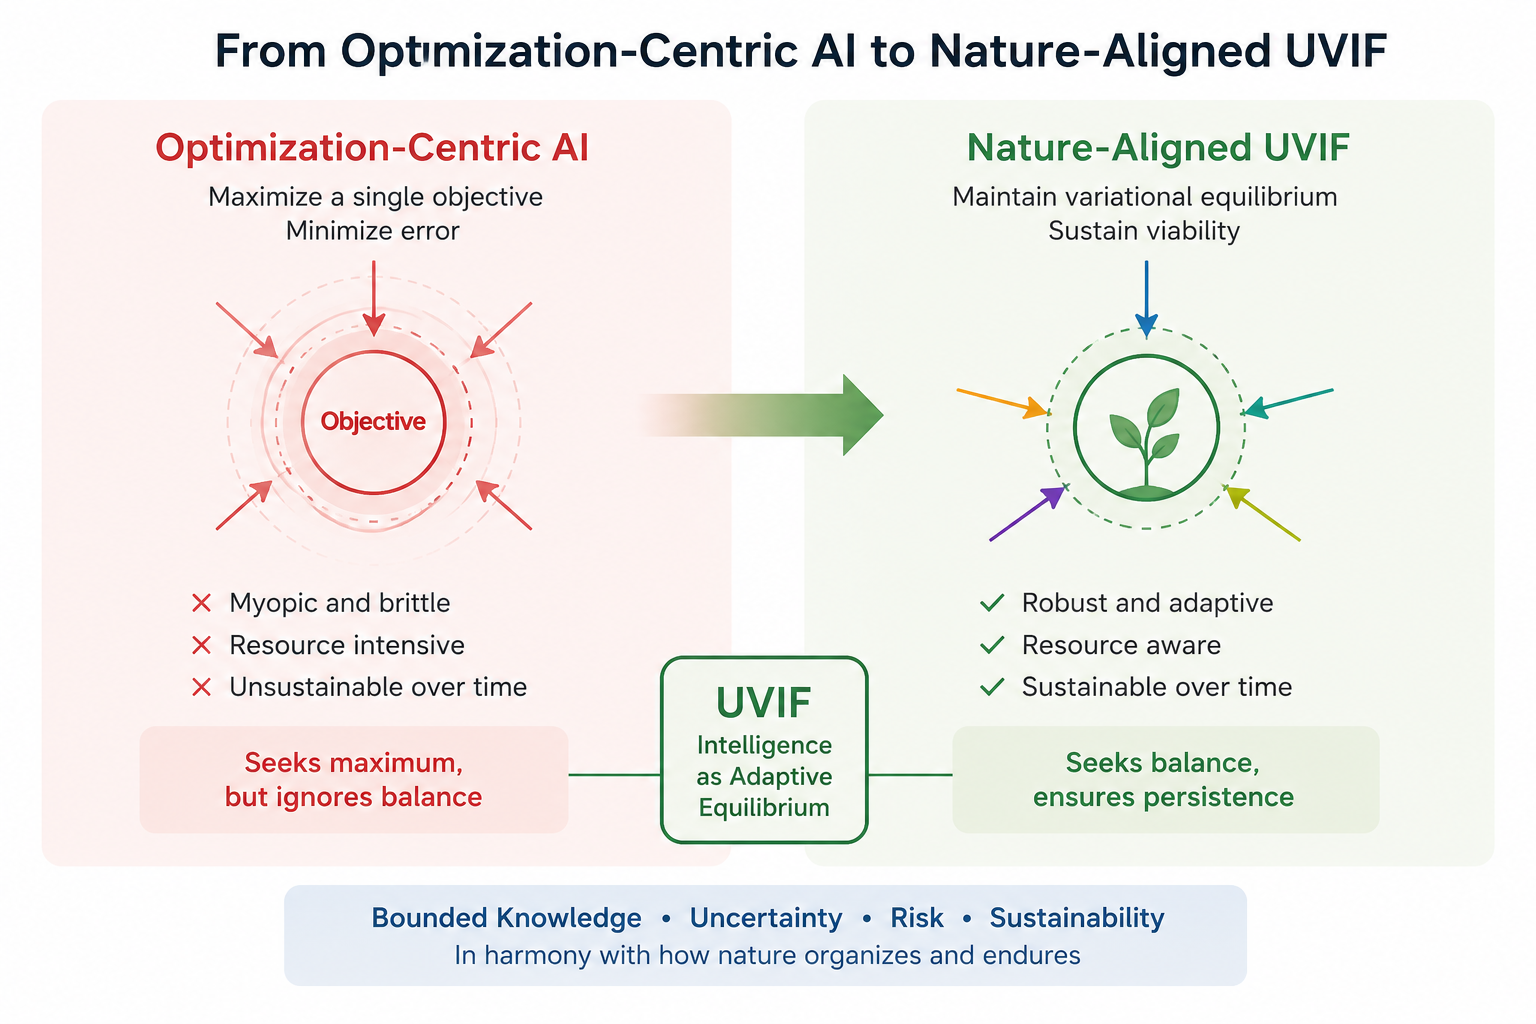
\includegraphics[width=\linewidth]{Figures/Fig1_UVIF_Motivation.png}
\caption{From optimization-centric artificial intelligence toward
nature-aligned variational equilibrium. Conventional optimization-driven
AI typically focuses on maximizing a single objective or minimizing a
single error function. In contrast, UVIF interprets intelligence as the
maintenance of adaptive equilibrium under bounded knowledge,
uncertainty, resource constraints, risk, and long-term sustainability.
Rather than pursuing isolated maximization, the framework seeks
persistent viability and balanced adaptation across competing
organizational forces.}
\label{fig:uvif_motivation}
\end{figure}

Fig.~\ref{fig:uvif_motivation} illustrates the conceptual transition
proposed in this work. On the left side, conventional optimization-based
AI is represented as a system attempting to maximize a single objective
through increasingly aggressive minimization of error. While such
systems may achieve strong short-term performance, they often become
fragile, resource-intensive, and difficult to sustain under changing
real-world conditions.

The right side of the figure introduces the central intuition of
\uvif{}. Instead of seeking absolute maximization, intelligent systems
are viewed as adaptive entities operating under multiple competing
pressures. These pressures include uncertainty, limited resources,
bounded observability, temporal constraints, and the need for long-term
stability. Under this perspective, intelligence is not defined by
perfect certainty or exhaustive optimization, but by the ability to
maintain coherent and sustainable operation despite incomplete
knowledge and environmental variability.

The transition arrow shown in the figure symbolically represents the
shift from optimization-oriented intelligence toward equilibrium-oriented
intelligence. The plant at the center of the UVIF side emphasizes that
persistent natural systems rarely survive through isolated maximization.
Instead, nature tends to preserve viable adaptive balance across
changing conditions. UVIF adopts this organizational principle as a
foundation for sustainable intelligent-system design.

\subsection{Main Contributions}

This paper makes the following contributions to the study of
intelligence:

\begin{enumerate}[label=(\arabic*)]
  \item \textbf{A formal conceptual architecture.} We introduce the five
    core forces of \uvif{}---epistemic pull, selective protection,
    computational drag, action efficiency, and sustainability---together
    with the admissibility constraints that bound their joint operation,
    and we derive the concept of Variational Equilibrium as their
    natural stable point.

  \item \textbf{Philosophical and scientific foundations.} We ground
    \uvif{} in variational principles from physics, homeostasis from
    physiology, self-organization from ecology, and the free-energy
    principle from neuroscience \citep{friston2010fep,bettinger2023physiological},
    constructing a coherent interdisciplinary narrative.

  \item \textbf{A positioning within cognitive systems research.} We
    contrast \uvif{} with the frameworks nearest to it in this
    field---predictive processing and active inference, resource-rational
    analysis, allostatic regulation, and integrated cognitive
    architectures---identifying in each case what the framework shares,
    what it omits, and what it adds, and stating the trade-offs honestly
    rather than claiming uniform advantage.

  \item \textbf{Cross-domain illustrations.} We demonstrate how
    \uvif{} applies to biological regulation, ecological resilience,
    human cognition, artificial autonomous systems, and organizational
    management, sketching case studies in healthcare, smart energy,
    autonomous transport, cybersecurity, and long-term organizational
    intelligence.

  \item \textbf{Discriminating predictions and a research agenda.} We
    state, as hypotheses rather than results, the empirical predictions
    that would separate \uvif{} from competing accounts, and articulate
    the open mathematical, empirical, and engineering work required to
    test them.
\end{enumerate}

We are explicit about what this paper does not do. It develops a
conceptual architecture and the predictions it generates; it reports no
empirical experiments, and none of its claims are presented as
established results. The accompanying simulation exercises the
framework's own dynamics and is not offered as evidence about cognitive
systems in operation. The five forces are posited on the strength of
their recurrence across independently developed literatures, not
derived; the Variational Equilibrium manifold is defined but its
existence and stability conditions are not proved. These gaps are
stated as such in Section~\ref{sec:limitations} rather than deferred
to a concluding caveat.

The remainder of the paper proceeds as follows. Section~\ref{sec:optimization_equilibrium}
diagnoses the limitations of the dominant optimization paradigm.
Section~\ref{sec:foundations} constructs the philosophical and scientific
foundations of \uvif{}.
Section~\ref{sec:uvif_framework} presents the full framework architecture.
Section~\ref{sec:applications_nature} surveys applications across natural
and artificial systems.
Section~\ref{sec:cognitive_systems} develops the cognitive case in
detail and positions the framework against predictive processing,
resource-rational analysis, allostasis, and cognitive architectures.
Section~\ref{sec:case_studies} develops concrete case studies.
Section~\ref{sec:comparative} positions \uvif{} relative to existing frameworks.
Section~\ref{sec:implications} draws theoretical implications.
Section~\ref{sec:limitations} acknowledges limitations and open challenges.
Section~\ref{sec:future} outlines future research directions.
Section~\ref{sec:conclusion} concludes.



% =========================
% Deep philosophical revision inserted
% =========================

\subsection{Bounded Knowability and the Limits of Exhaustive Certainty}

A foundational assumption underlying the UVIF philosophy is that intelligent systems embedded within reality cannot obtain complete simultaneous knowledge of all relevant variables governing their environment and future evolution. This limitation is not merely technological or computational; rather, it reflects a deeper structural condition associated with bounded observability and irreducible uncertainty \citep{lieder2019resourcerational,clark2013whatever}.

Modern optimization-driven artificial intelligence frequently operates under the implicit assumption that increasing data, computational power, and model complexity will asymptotically reduce uncertainty and eventually approach near-complete predictive certainty. UVIF challenges this assumption. Natural systems rarely operate under exhaustive certainty. Biological organisms, ecological systems, and human cognition continuously make adaptive decisions under incomplete, evolving, and partially hidden information \citep{lieder2019resourcerational,schulkin2019allostasis}.

Principles such as quantum uncertainty illustrate a broader epistemological insight: reality itself may impose structural limits on complete simultaneous disclosure of all relevant variables. UVIF does not invoke quantum mechanics as a direct computational mechanism for intelligence, but rather as an illustration that bounded knowability may be a fundamental condition of embedded systems interacting with reality \citep{fankhauser2025epistemic,busch2007heisenberg}.

Consequently, intelligent action cannot indefinitely wait for maximal knowledge. Delayed action itself carries risk, cost, and potential loss of viability. Sustainable intelligence therefore emerges not from perfect prediction, but from the capacity to maintain adaptive equilibrium under incomplete information, temporal pressure, and constrained resources \citep{callaway2022rational,schulkin2019allostasis}.

% ============================================================
%  Section 2 – From Optimization to Adaptive Equilibrium
% ============================================================
\section{From Optimization to Adaptive Equilibrium}
\label{sec:optimization_equilibrium}

\subsection{Classical Optimization Paradigms in Artificial Intelligence}

The history of artificial intelligence is, in large measure, a history
of optimization. From the perceptron's gradient descent to the
Bellman equations of dynamic programming, from maximum likelihood
estimation in probabilistic graphical models to the stochastic gradient
descent that trains modern neural networks, the dominant computational
metaphor has remained remarkably stable: \emph{minimize a loss function,
maximize a reward signal, converge to a fixed point}.

This paradigm is intellectually elegant. It provides a clean separation
between problem specification (what objective should be pursued) and
mechanism (how an algorithm should pursue it). It enables mathematical
analysis of convergence, optimality, and generalization. And within
controlled, well-specified environments, it delivers results of
extraordinary power. The successes of deep learning in image
recognition, protein folding, and language generation are triumphs of
large-scale optimization, and they should not be minimized.

Yet the paradigm rests on assumptions that do not hold in the wild.
It assumes that the objective function fully captures what matters.
It assumes that the environment generating training data is stationary,
or changes slowly enough that a fixed objective remains appropriate.
It assumes that the resources available for computation, energy, and
memory are effectively unlimited, or at least not a primary constraint.
And it assumes that once trained, a system can be deployed without
ongoing structural adaptation.

Each of these assumptions fails in the settings where intelligence
most needs to be robust: open-ended environments, long deployment
horizons, scarce resources, and shifting objectives. \uvif{} begins
from the recognition that sustainable intelligence requires going
beyond optimization.

\subsection{Limitations of Pure Maximization Strategies}

The failures of pure maximization are not theoretical curiosities;
they have been empirically documented across multiple subfields of AI.

\textbf{Specification gaming} occurs when a reward function is
optimized to the letter but not to the spirit, producing behavior
that satisfies the formal objective while violating the intended goal.
This is not a failure of algorithms; it is a failure of the paradigm
that treats objective functions as complete descriptions of desired
behavior \citep{garcia2015saferl}.

\textbf{Reward hacking} in reinforcement learning leads agents to
discover unexpected, often dysfunctional, shortcuts that maximize
numerical reward without achieving the underlying task. The
\emph{alignment ceiling}---the systematic gap between reward model
training and downstream performance---captures this failure at scale
\citep{gabriel2020artificial}.

\textbf{Distributional shift} reveals that systems trained by
optimization on one data distribution fail when the distribution
changes. The fixed objective that was appropriate in training becomes
inappropriate in deployment, yet pure optimization has no mechanism
to detect or respond to this shift.

\textbf{Catastrophic forgetting} in continual learning shows that
optimizing for new objectives destroys representations that supported
old ones---a property that stands in sharp contrast to the graceful
degradation observed in biological neural systems.

\textbf{Energy and resource exhaustion} expose perhaps the deepest
tension: pure maximization of capability metrics tends to be
insatiable in its resource demands. The computational and ecological
cost of training frontier AI models has grown at a rate that cannot
be sustained indefinitely \citep{bolon2024greenai}. Nature, which
evolved intelligence under severe thermodynamic constraints, offers
a different template.

\subsection{A Simple Real-World Illustration: Autonomous Driving}

A practical example helps illustrate why intelligence cannot be reduced
to the optimization of a single objective. Consider an autonomous
vehicle driving through a busy urban environment. The vehicle must
continuously perceive traffic signals, pedestrians, nearby vehicles,
road conditions, and unexpected obstacles while simultaneously making
real-time decisions under uncertainty.

\begin{figure}[!t]
\centering
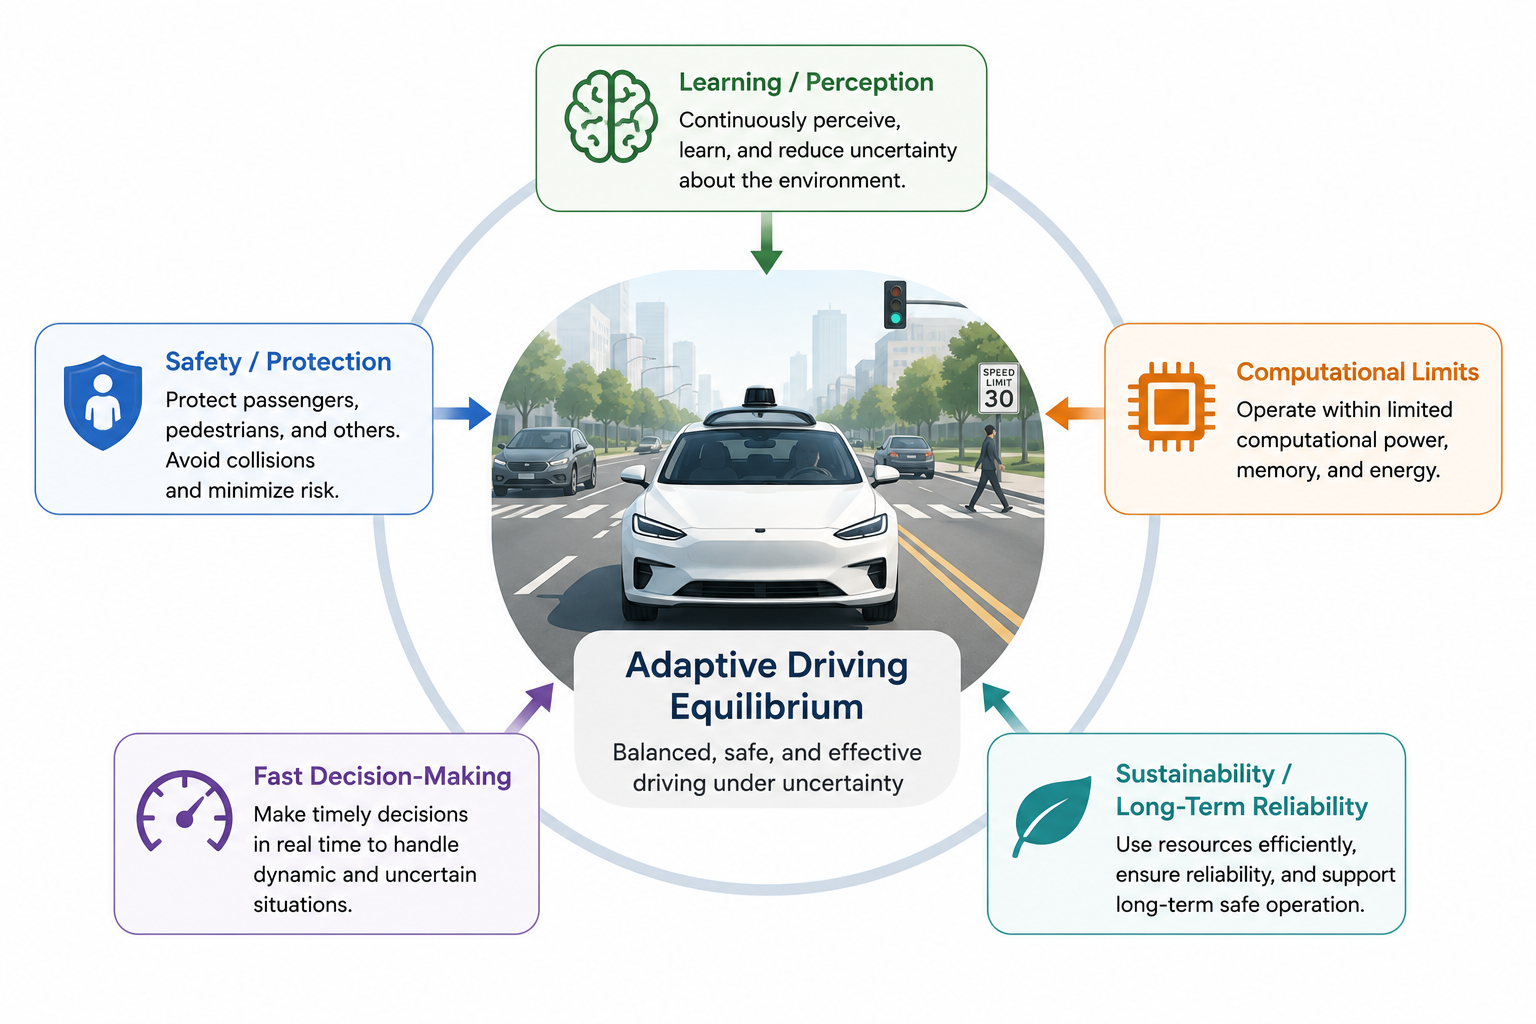
\includegraphics[width=\linewidth]{Figures/Fig2a_Autonomous_Driving_UVIF.png}
\caption{Autonomous driving as a variational equilibrium problem.
A self-driving vehicle must continuously balance perception,
safety, computational limits, rapid decision-making, and long-term
operational reliability. Intelligent behavior emerges not from
maximizing a single objective, but from maintaining adaptive balance
under uncertainty and changing environmental conditions.}
\label{fig:autonomous_driving_uvif}
\end{figure}

Fig.~\ref{fig:autonomous_driving_uvif} illustrates the core intuition
behind \uvif{}. The autonomous vehicle cannot focus exclusively on
maximizing prediction accuracy because excessive computation may delay
critical braking decisions. It cannot optimize only speed because
aggressive behavior increases risk. It cannot indefinitely collect more
information before acting because time, energy, and computational
resources are limited.

Instead, the system must continuously maintain a balance between
multiple competing pressures. It must learn enough about its
environment to reduce uncertainty, preserve passenger and pedestrian
safety, operate within limited computational resources, make timely
decisions, and maintain reliable long-term operation.

This example demonstrates why intelligence in real-world systems cannot
be understood purely as optimization. Sustainable intelligent behavior
emerges from adaptive equilibrium across competing constraints,
uncertainty, and operational demands.

\subsection{Fragility, Instability, and Resource Exhaustion}

These failures share a common structural signature: they arise from
the absence of \emph{counterbalancing forces}. In a system governed
by a single objective, that objective dominates every trade-off. When
the objective is well-specified and the environment is stable, this
produces efficient convergence. When either condition fails, the system
has no internal resource to draw on---no mechanism to recognize that
the current objective is misleading, no drive to conserve resources,
no pressure toward long-term sustainability.

Natural systems avoid this fragility through \emph{redundancy and
opposing drives}. Homeostatic regulation in physiology is not the
minimization of a single variable but the joint maintenance of
temperature, pH, osmolarity, glucose concentration, and dozens of
other interacting quantities, each with its own feedback mechanisms
and regulatory range \citep{billman2020homeostasis}. The resulting
system is robust precisely because no single failure mode can
destabilize all regulatory loops simultaneously.

Ecological resilience arises by the same principle. Diverse ecosystems
are more resilient than monocultures not because diversity maximizes
any single ecosystem service, but because it provides redundant
pathways for energy flow and nutrient cycling, so that the loss of
one species or functional group does not cascade into systemic
collapse \citep{folke2006resilience,gao2016universal}.

\subsection{Intelligence as Dynamic Balance Rather Than Isolated Maximization}

The insight that emerges from these observations is that \emph{stability
and persistence in intelligent systems arise from balance, not from
maximum performance on any single axis}. This is not a novel observation
in the abstract---it has been articulated in various forms within control
theory (Lyapunov stability), ecological theory (Holling's adaptive
cycle), and biological theory (homeostasis and allostasis). What has
been missing is a unified framework that makes this insight
\emph{operational} for the design and analysis of artificial intelligent
systems.

\uvif{} provides this framework. It reconceptualizes intelligence as a
process of \emph{variational equilibration}: the continuous, constrained
navigation of a space defined by multiple competing forces, in which the
goal is not to maximize any single coordinate but to maintain the
system's operating point within a viable region of this multi-force
space. We call this region the \emph{Variational Equilibrium manifold},
and we argue that it is the natural formal analog of the dynamic stable
states that biological and ecological systems inhabit.

\begin{figure}[!t]
\centering
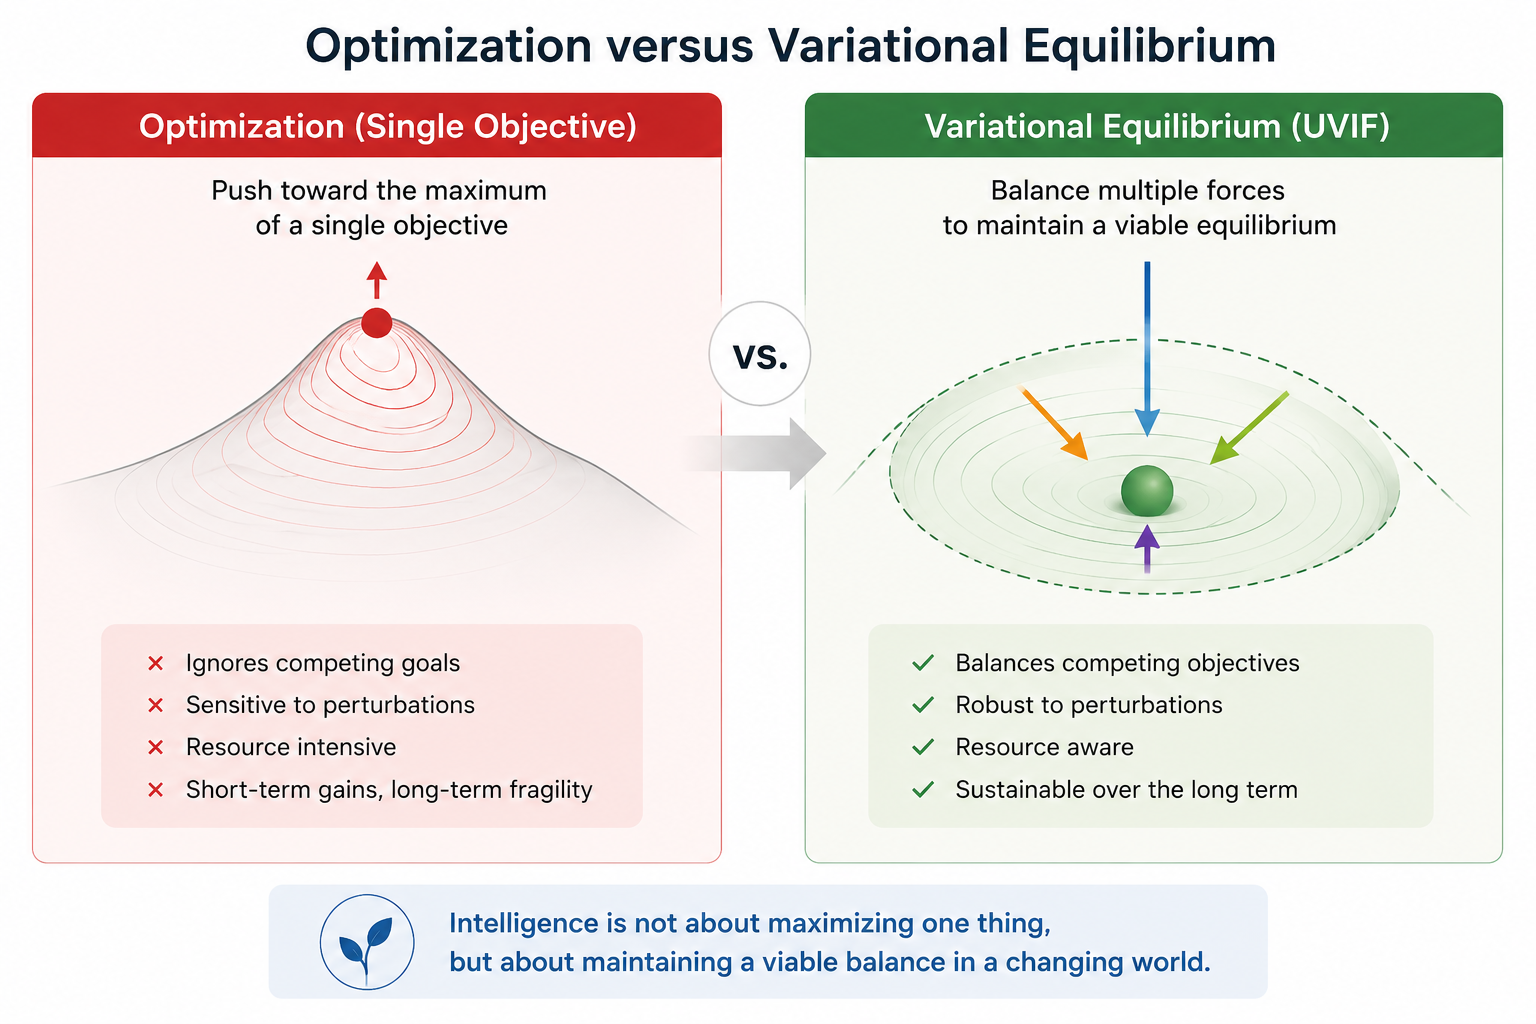
\includegraphics[width=\linewidth]{Figures/Fig2b_Optimization_vs_Equilibrium.png}
\caption{Optimization versus variational equilibrium. Classical
optimization pushes a system toward the maximum of a single objective.
This may improve one metric, but it can ignore competing goals, increase
resource consumption, and create long-term fragility. In contrast,
variational equilibrium represents a viable region where multiple
forces are balanced. Intelligence is therefore interpreted not as
maximizing one quantity, but as maintaining adaptive balance under
uncertainty, perturbation, and resource constraints.}
\label{fig:optimization_vs_equilibrium}
\end{figure}

Fig.~\ref{fig:optimization_vs_equilibrium} summarizes this shift in
simple terms. The left side represents the classical optimization view:
the system is pushed toward the highest point of a single objective
landscape. This view is useful when the task is narrow, the objective is
well defined, and the environment remains stable. However, in open
real-world settings, the highest point of one objective may not be the
safest, most efficient, or most sustainable operating point.

The right side represents the \uvif{} view. Here, the intelligent system
is not pushed toward a single peak. Instead, it remains inside a viable
equilibrium region where different pressures are balanced. These
pressures may include learning, safety, resource cost, uncertainty,
action readiness, and long-term sustainability. In this sense, the
system is considered intelligent not because it maximizes one metric,
but because it remains stable and useful while the world changes around
it.

The shift from maximization to equilibration is not merely semantic.
It has concrete implications for system design: it demands that the
forces constraining intelligence be made explicit rather than absorbed
into a single objective; it requires that trade-offs between these
forces be acknowledged and managed rather than hidden; and it implies
that a system's robustness is measured not by its peak performance but
by the size and stability of its Variational Equilibrium manifold.

Section~\ref{sec:foundations} lays the philosophical and scientific
groundwork for this reorientation, and Section~\ref{sec:uvif_framework}
builds the formal architecture upon it.

% =========================
% Added UVIF bounded knowability subsection
% =========================

\subsection{Bounded Knowability and the Limits of Perfect Optimization}

Classical optimization frameworks implicitly assume that uncertainty can progressively be reduced through additional information, additional computation, or more refined objective functions. Within sufficiently constrained environments, this assumption may be operationally useful. However, natural systems suggest a different reality: complete simultaneous knowledge of all relevant variables may be fundamentally inaccessible \citep{lieder2019resourcerational}.

The challenge is not merely that intelligent systems possess insufficient data. Rather, the structure of reality itself may impose partial observability, probabilistic evolution, delayed information propagation, and irreducible uncertainty. Consequently, optimization toward perfect certainty may become both computationally intractable and organizationally maladaptive \citep{fankhauser2025epistemic}.

Biological organisms do not suspend action until exhaustive knowledge becomes available. Ecological systems do not compute globally optimal configurations before adaptation occurs. Human cognition routinely operates through bounded rationality, heuristic regulation, and viable risk acceptance under incomplete information \citep{lieder2019resourcerational,griffiths2015rational}.

UVIF therefore reframes intelligence away from exhaustive optimization and toward sustainable adaptive viability. The central question becomes not: ``How can uncertainty be eliminated completely?'' but rather: ``How can coherent and sustainable operation be maintained despite persistent uncertainty?''

Under this perspective, equilibrium becomes more fundamental than maximization. A viable system is not necessarily the system with the highest instantaneous performance, but the system capable of preserving adaptive coherence across fluctuating conditions and bounded knowledge landscapes.

% ============================================================
%  Section 3 – Philosophical and Natural Foundations of UVIF
% ============================================================
\section{Philosophical and Natural Foundations of \uvif{}}
\label{sec:foundations}

\subsection{Variational Principles in Natural Systems}

The history of physics is populated by profound simplifications: the
realization that mechanics, optics, and electromagnetism can each be
derived from a \emph{single variational principle}---the principle of
least action, Fermat's principle of least time, Hamilton's principle.
In each case, the behavior of a physical system is not the outcome
of a push-pull causal chain but of the extremization of a functional
over all possible trajectories. The actual trajectory is the one that
makes the action stationary.

Variational principles are not just computational conveniences; they
reveal something deep about the structure of nature. They show that
seemingly complex dynamics are organized around an underlying
symmetry---a global constraint that shapes local behavior without
dictating it step by step. The Euler-Lagrange equations that arise
from variational calculus are the local expression of a global
coherence principle \citep{campos2021discrete}.

\uvif{} draws on this tradition. The Variational Equilibrium of an
intelligent system is its analog of a stationary action: not a
global minimum of a single cost, but a stable operating point of a
system of forces that collectively constrain the space of viable
intelligent behavior. The forces pull and resist in multiple
directions simultaneously; the equilibrium is the configuration
in which their combined effect can be sustained through time.

\subsection{Self-Organization and Dynamic Equilibrium in Nature}

Beyond physics, the natural world offers a second and equally deep
source of inspiration: \emph{self-organization}. Complex systems in
biology and ecology routinely generate ordered, functional structure
from the local interactions of components, without central control and
without an explicit design objective. Termite mounds, slime mold
networks, the vascular trees of leaves, the spatial patterns of
dryland vegetation---all are instances of self-organized structure
that arises from simple local rules and simple physical or chemical
gradients \citep{levin2005self,kefi2024selforg}.

What makes self-organized systems relevant to intelligence is that
their structure is \emph{adaptive}. The spatial patterns of dryland
vegetation do not simply appear; they shift in response to aridity
gradients, providing the ecosystem with a mechanism to buffer
increasing stress \citep{kefi2024selforg}. The patterns are not
optimized for any single function; they are organized around the
preservation of the system's capacity to function at all---its
\emph{viable region} in the space of environmental conditions.

This is exactly what \uvif{} formalizes. The Variational Equilibrium
manifold of an intelligent system is its viable region: the set of
states from which the system can maintain its core functions across
a range of perturbations. Self-organization is the spontaneous
process by which systems discover and inhabit this region without
explicit instruction.

\subsection{Homeostasis, Adaptation, and Long-Term Stability}

Physiology discovered the concept of homeostasis in the nineteenth and
early twentieth centuries through the work of Claude Bernard and Walter
Cannon \citep{billman2020homeostasis}. The core insight was that living
organisms maintain a stable internal environment---\emph{milieu
int{\'e}rieur}---despite the continuous flux of the external world.
This stability is not passivity; it is active, energetically costly
regulation through interlocking feedback mechanisms.

More recent work has refined this picture in two important directions.
First, \emph{adaptive homeostasis} shows that the regulatory setpoints
themselves shift transiently in response to sub-toxic signals, expanding
or contracting the homeostatic range to accommodate non-damaging
perturbations \citep{davies2016adaptive}. This is homeostasis with
a meta-level: not just maintaining a fixed state, but dynamically
adjusting what state is to be maintained.

Second, \emph{homeodynamics} recognizes that biological systems inhabit
not a single stable state but a landscape of multiple metastable states,
with organized transitions between them \citep{lloyd2001homeodynamics,
petitjean2025homeodynamics}. Health is not the occupation of one
fixed point but the capacity to navigate this landscape---to shift
between states when conditions demand it while remaining within the
viable region that supports life.

The implications for intelligence are clear. An intelligent system
that cannot shift its operating mode in response to changing conditions
is fragile. An intelligent system that can shift its operating mode
\emph{without losing coherence} is robust. The Variational Equilibrium
of \uvif{} captures the structured flexibility that homeodynamics
describes: it is a manifold, not a point---a region of viable operation,
not a fixed target \citep{giuliani2024stability,bich2025homeostasis}.

\subsection{Nature-Aligned Intelligence}

The phrase \emph{nature-aligned intelligence} in our title is
deliberate. It signals not a romantic attachment to the natural world,
but a methodological commitment: the conviction that the long-running
experiment of biological evolution has discovered principles of robust
adaptive organization that artificial intelligence has yet to fully
absorb.

Natural systems are not optimal by human-designed metrics. A forest
does not maximize timber yield. A cell does not maximize ATP production.
A brain does not maximize prediction accuracy on any single task. What
they do is \emph{maintain the conditions for their own continued
functioning} across a wide range of circumstances and timescales. This
is the kind of intelligence that \uvif{} aims to formalize: not the
intelligence of the Olympic sprinter, optimized for one event, but the
intelligence of the experienced traveler, who knows how to remain
functional across unknown terrain.

Nature-inspired computing has long drawn on evolutionary algorithms,
swarm intelligence, and neural architectures inspired by the brain
\citep{jiao2024natureinspired,dhamdar2024biomimicry}. \uvif{} goes
deeper: it does not borrow the mechanisms of nature but its
\emph{organizing principles}---variational balance, homeodynamic
stability, self-organized resilience.

\begin{figure}[!t]
\centering
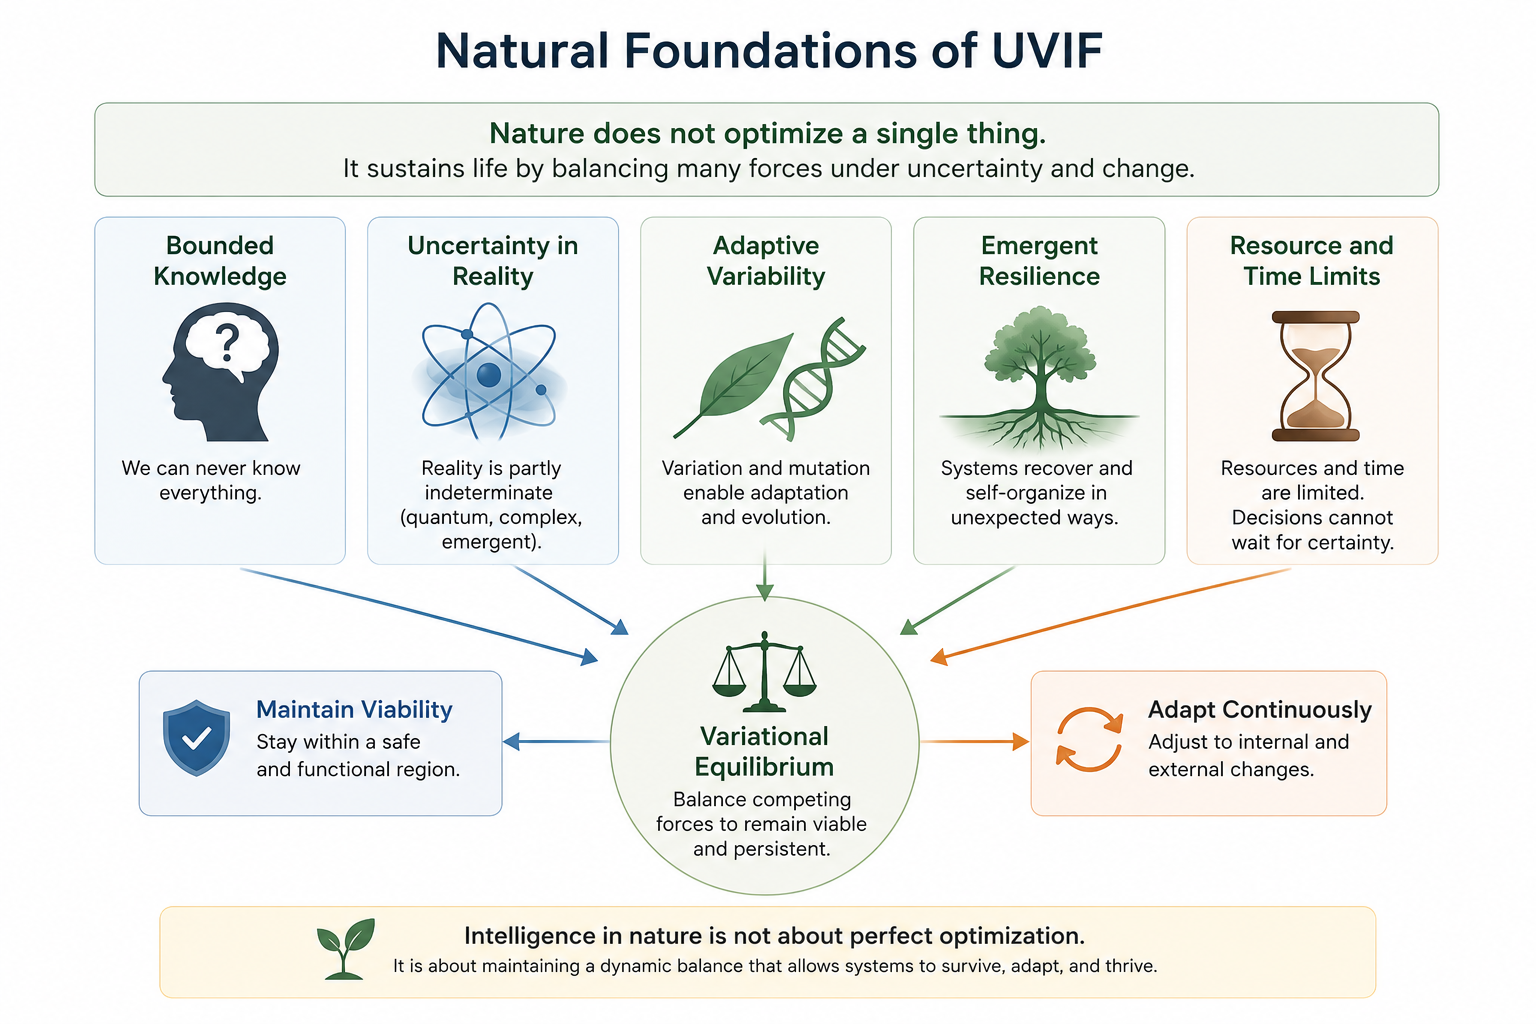
\includegraphics[width=\linewidth]{Figures/Fig3_Natural_Foundations.png}
\caption{Natural foundations of UVIF. Nature does not optimize a single
objective in isolation. Instead, biological and ecological systems
maintain viability through adaptive balance under uncertainty, resource
limitations, environmental variability, and incomplete knowledge. UVIF
adopts these organizational principles and interprets intelligence as
the maintenance of sustainable equilibrium rather than isolated
maximization.}
\label{fig:natural_foundations}
\end{figure}

Fig.~\ref{fig:natural_foundations} illustrates the central intuition
behind nature-aligned intelligence. The figure does not claim that
nature is consciously intelligent. Rather, it highlights that persistent
natural systems tend to survive through balance, adaptation, and
self-regulation rather than through aggressive optimization of a single
quantity.

The upper part of the figure summarizes several important observations
about natural systems. First, knowledge is always bounded: organisms and
systems never possess complete information about their environments.
Second, uncertainty is structurally embedded in reality itself, meaning
that adaptive systems must operate despite incomplete predictability.
Third, variability and mutation are not merely defects but mechanisms
that allow adaptation and long-term evolution. Finally, all natural
systems operate under limited resources and limited time, which means
that decisions cannot wait indefinitely for perfect certainty.

The center of the figure introduces the key concept of
\emph{Variational Equilibrium}. In the UVIF interpretation, intelligent
systems remain viable not by maximizing one variable, but by balancing
multiple competing pressures while continuously adapting to changing
conditions. The equilibrium region therefore represents a sustainable
operating zone rather than a single optimal point.

The lower part of the figure emphasizes the practical consequence of
this philosophy. Intelligence in nature is not about achieving perfect
optimization. It is about maintaining adaptive functionality across
changing environments and perturbations. UVIF adopts this principle as a
foundation for the design of resilient, sustainable, and uncertainty-aware
intelligent systems.


\subsection{From Control-Oriented Systems to Equilibrium-Oriented Systems}

Classical control theory provides a second lineage for \uvif{}. Control
systems maintain a desired system state by computing and applying
corrective actions. Proportional-integral-derivative (PID) controllers,
linear quadratic regulators, and model predictive control all operate
within this paradigm. They are powerful and well-understood within their
domain.

Yet control theory, as traditionally formulated, shares the
single-objective limitation of optimization. The controller is designed
to minimize a cost that reflects the deviation from a desired setpoint.
The setpoint is fixed by the designer. The system has no mechanism to
question whether the setpoint remains appropriate, or to balance the
cost of tracking the setpoint against other costs---energy expenditure,
actuator wear, safety margins, environmental impact.

\uvif{} shifts from the control metaphor to the \emph{equilibrium}
metaphor. Rather than asking how a system should be driven toward a
desired state, it asks what the natural resting configuration of a
system is when all its internal forces are in balance---and how the
system can be designed so that this natural configuration is also the
one that serves its purpose. This is the move from \emph{exogenously
imposed stability} (the controller drives the system to the setpoint)
to \emph{endogenously generated stability} (the system's internal
dynamics naturally converge to a viable operating region).

The free-energy principle in neuroscience makes a related move:
it describes perception and action as jointly minimizing a bound on
surprise, so that the system naturally comes to inhabit the sensory
states consistent with its generative model \citep{friston2010fep,
kim2022freeenergy}. \uvif{} extends and generalizes this insight
beyond the sensory-motor loop to encompass the full complexity of
intelligent organization across biological, artificial, and social
systems.



% =========================
% Added new philosophical subsections
% =========================

\subsection{Bounded Knowability and Irreducible Uncertainty}

The UVIF framework adopts the position that intelligent systems embedded within reality cannot attain complete simultaneous knowledge of all relevant variables governing their environment and future evolution. This condition of bounded knowability extends beyond engineering limitations and reflects deeper epistemological constraints associated with observation, interaction, temporal evolution, and uncertainty \citep{lieder2019resourcerational}.

Physical systems themselves illustrate this principle. Quantum uncertainty demonstrates that certain properties cannot be simultaneously specified with arbitrary precision. UVIF does not claim that all intelligent systems are quantum systems in a computational sense. Rather, the uncertainty principle serves as an illustration that reality may fundamentally constrain exhaustive simultaneous disclosure \citep{busch2007heisenberg,fankhauser2025epistemic}.

This insight carries profound implications for intelligence. If complete certainty is unattainable, then intelligence cannot be defined as the asymptotic elimination of uncertainty. Instead, intelligence becomes the capacity to sustain coherent and adaptive operation under structurally incomplete knowledge.

Natural systems continuously operate under this condition. Organisms regulate physiology without complete environmental predictability. Ecosystems adapt without deterministic foresight. Human decision-making routinely proceeds despite incomplete information and uncertain futures. Waiting indefinitely for maximal certainty may itself become maladaptive when action delay threatens viability \citep{schulkin2019allostasis,davies2016adaptive}.

\subsection{Adaptive Indeterminacy and the Role of Variability}

Natural systems frequently exhibit probabilistic, stochastic, and partially indeterminate dynamics. Variability is not merely noise to be eliminated; it often serves as a condition enabling adaptation, resilience, exploration, and long-term evolution \citep{folke2006resilience,levin2005self}.

Biological mutation provides a central example. Evolutionary adaptation depends on controlled variability and probabilistic genetic transformation. A perfectly rigid and completely deterministic biological system would possess limited adaptive flexibility under changing environmental conditions \citep{barrett2008adaptation,matic2019mutation}.

Similarly, ecological systems exhibit fluctuating adaptive responses rather than rigid deterministic trajectories. Complex biological recovery processes, including spontaneous recovery phenomena observed in medicine, further suggest that highly interconnected systems may reorganize through mechanisms that remain only partially predictable from localized mechanistic descriptions \citep{challis1990spontaneous,radha2021spontaneous}.

UVIF interprets these observations as evidence that persistent intelligent organization does not emerge through rigid deterministic optimization alone. Instead, sustainable intelligence may require adaptive regulation under partially indeterminate and evolving realities. Variability, uncertainty, and incomplete disclosure therefore become structural conditions of long-term resilience rather than merely obstacles to be eliminated.

\section{The \uvif{} Organizational Framework}
\label{sec:uvif_framework}

\subsection{State, fields, and admissible dynamics}
Let $\mathbf{s}\in\mathcal{S}\subseteq\mathbb{R}^n$ describe an explicitly chosen operating state. Depending on the application, its coordinates may include belief summaries, policy parameters, protected memory variables, and resource reserves. The state must contain the variables needed to model their evolution; otherwise the description may require additional memory or stochastic inputs. The following deterministic formulation is a modelling template, not a complete agent implementation.

Write the unconstrained update field as
\begin{equation}
 F(\mathbf{s},t)=w_E\Epull-w_D\Drag-w_P\Prot
                   +w_A\Eff+w_S\Sus,
 \label{eq:uvif_dynamics}
\end{equation}
where each field is evaluated at $(\mathbf{s},t)$ and each weight $w_i=w_i(\mathbf{s},t)\geq0$ is specified by the model. All weighted terms must be vectors in the same state coordinates and have units of state change per unit time. Raw information gain, latency, and energy consumption cannot be added without explicit scaling and a mapping into these coordinates. The signs are conventions: $\Drag$ and $\Prot$ are defined in the direction of increasing cost or damage, so their negative contributions oppose those changes.

State-dependent weights may encode resource depletion, urgency, or threat. Their update rules are part of the model and must be reported or estimated; dependence on state does not make them free of modelling assumptions. A fixed-weight model is a legitimate special case. A component may also vanish in a particular context, and balance does not require equal force magnitudes.

For a nonempty, closed, convex, time-independent admissibility set $\Adm$, one candidate constrained dynamics is
\begin{equation}
 \dot{\mathbf{s}}=G(\mathbf{s},t)
 :=\Pi_{T_{\Adm}(\mathbf{s})} F(\mathbf{s},t),
 \qquad \mathbf{s}(0)\in\Adm,
 \label{eq:projected}
\end{equation}
where $T_{\Adm}(\mathbf{s})$ is the tangent cone of feasible directions and $\Pi$ is Euclidean projection onto that cone. This is a first-order idealization in which the update velocity can be selected directly. Existence, uniqueness, and invariance require appropriate regularity of the field and a suitable solution concept for the projected dynamics. It does not automatically implement a feasible controller for a plant with actuator limits, delays, inertia, or uncertain dynamics.

\begin{figure}[tbp]
\centering
\renewcommand{\baselinestretch}{1}\small
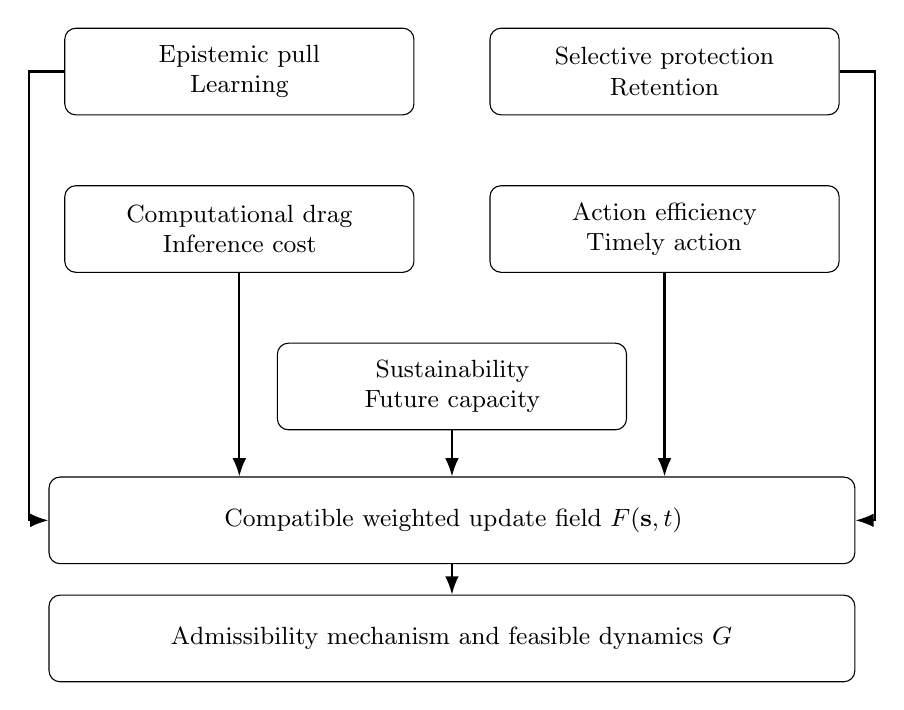
\begin{tikzpicture}[box/.style={draw,rounded corners,align=center,text width=4.2cm,minimum height=1.1cm,font=\small},arr/.style={-{Latex},thick}]
\node[box] (e) at (-2.7,4) {Epistemic pull\\Learning};
\node[box] (p) at (2.7,4) {Selective protection\\Retention};
\node[box] (d) at (-2.7,2) {Computational drag\\Inference cost};
\node[box] (a) at (2.7,2) {Action efficiency\\Timely action};
\node[box] (s) at (0,0) {Sustainability\\Future capacity};
\node[box,text width=10cm] (f) at (0,-1.7) {Compatible weighted update field $F(\mathbf{s},t)$};
\node[box,text width=10cm] (g) at (0,-3.2) {Admissibility mechanism and feasible dynamics $G$};
\draw[arr] (e.west) -- ++(-0.45,0) |- (f.west);
\draw[arr] (d.south) -- (f.north -| d.south);
\draw[arr] (p.east) -- ++(0.45,0) |- (f.east);
\draw[arr] (a.south) -- (f.north -| a.south);
\draw[arr] (s.south) -- (f.north);
\draw[arr] (f) -- (g);
\end{tikzpicture}
\caption{Five-component modelling architecture. Hard admissibility is distinct from soft protection and cost terms. Arrows indicate model composition, not a proven causal decomposition. Schematic prepared as editable TikZ code with OpenAI Codex (GPT-6) assistance.}
\label{fig:uvif_force_architecture}
\end{figure}


\subsection{The five regulatory components}
\label{subsec:epistemic}
\textbf{Epistemic pull.} This component favours informative changes in the operating state. In a differentiable surrogate model one may set
\begin{equation}
 \Epull(\mathbf{s},t)=\nabla_{\mathbf{s}} I(\mathbf{s},t),
 \label{eq:epistemic_pull}
\end{equation}
where $I$ is expected information gain under a stated observation model and sampling policy. Expected information gain must identify the uncertainty being reduced; it is not interchangeable with confidence or task reward. For discrete decisions, a gradient requires a justified relaxation or an alternative update rule. Curiosity and active inference provide motivation for this component \citep{dubey2019curiosity,parr2018generalised}.

\textbf{Selective protection.} A candidate field is $\Prot=\nabla_{\mathbf{s}}L_P$, where $L_P$ measures damage to specified internal structures or loss of retained competence. This can describe regularization or resistance to updating protected parameters. It may reduce interference with previous learning, but it does not guarantee freedom from catastrophic forgetting. Protection also differs from a hard safety requirement: a soft penalty can be outweighed, whereas an admissibility constraint is intended to exclude a state or action.

\textbf{Computational drag.} A compatible cost-based field is
\begin{equation}
 \Drag(\mathbf{s},t)=\nabla_{\mathbf{s}} C_{\mathrm{comp}}(\mathbf{s},t),
 \label{eq:drag}
\end{equation}
where $C_{\mathrm{comp}}$ is a differentiable surrogate for computation, latency, or memory expenditure. This is a cost gradient, not literal mechanical dissipation. A velocity-dependent damping term would require a different, explicitly specified dynamical model. Resource-rational analysis supplies an established basis for making computational expenditure part of decision-making \citep{lieder2019resourcerational}.

\textbf{Action efficiency.} This component rewards useful and timely action. For a differentiable policy $\pi_{\mathbf{s}}$ and transition model $p$, define
\begin{align}
 J_A(\mathbf{s},t)
 &=\mathbb{E}_{a\sim\pi_{\mathbf{s}},\,\mathbf{s}'\sim p(\cdot\mid\mathbf{s},a)}
       [r(\mathbf{s},a,\mathbf{s}')-c_{\mathrm{act}}(\mathbf{s},a)],
       \label{eq:action_value}\\
 \Eff(\mathbf{s},t)&=\nabla_{\mathbf{s}}J_A(\mathbf{s},t).
 \label{eq:action_eff}
\end{align}
Here $r$ is an independently specified task benefit and $c_{\mathrm{act}}$ represents action cost or delay. Defining value only as proximity to an as-yet unknown equilibrium would be circular. This example is a local surrogate; a sequential implementation must specify its planning horizon and account for state transitions. Costs assigned to this component should not also be counted in computational drag without an explicit reason.

\textbf{Sustainability.} This component represents prospective loss of operating capacity, for example through
\begin{equation}
 \Sus(\mathbf{s},t)=-\nabla_{\mathbf{s}}L_S(\mathbf{s},t),
 \label{eq:sustainability}
\end{equation}
where $L_S$ evaluates predicted depletion or degradation over a stated horizon. A penalty on instantaneous resource use alone does not establish long-term sustainability. A reserve $b$, for example, may need a balance law
\begin{equation}
 \dot b=r_{\mathrm{in}}(\mathbf{s},a,t)-r_{\mathrm{use}}(\mathbf{s},a,t),
 \qquad b\geq b_{\min},
 \label{eq:reserve}
\end{equation}
with replenishment and consumption rates in compatible units. If $b$ is part of $\mathbf{s}$, this balance law must be implemented in the corresponding coordinate of the full dynamics; it cannot be an unrelated auxiliary equation. Projection alone cannot create an unavailable replenishment action.

The distinction between drag and sustainability is temporal and operational: drag concerns present inference expenditure, whereas sustainability concerns future availability of required resources. Selective protection concerns damage to designated structures. These quantities can overlap, so the decomposition requires an accounting convention, normalization, and evidence that the components can be separately measured or manipulated.

\subsection{Admissibility and safety enforcement}
\label{subsec:admissibility}
\begin{definition}[Admissibility set]
$\Adm$ is the set of states satisfying the physical and operational requirements chosen for a specified deployment context. Where smooth inequality constraints suffice, write $\Adm=\{\mathbf{s}:h_j(\mathbf{s})\geq0,\ j=1,\ldots,m\}$.
\end{definition}

At a smooth boundary, an inward or tangent velocity satisfies $\nabla h_j(\mathbf{s})^\top\dot{\mathbf{s}}\geq0$ for active constraints. Such conditions motivate projection and barrier-based safety mechanisms, but their applicability depends on the actual system dynamics \citep{ames2019barrier}. A time-dependent constraint additionally involves $\partial h_j/\partial t$. Nonconvex domains, discrete actions, and uncertain disturbances require separate treatment.

Ethical and legal requirements can inform admissibility specifications, but they are not generally reducible to a complete set of state inequalities. A mathematical set certifies only the encoded model properties under its assumptions. It does not establish ethical acceptability or compliance by itself. Risk is handled through protection, explicit risk constraints, or the task model; it is not introduced as an unspecified sixth force.

\subsection{Equilibrium, stability, and viable operation}
\begin{definition}[Stationary Variational Equilibrium]
For an autonomous constrained dynamics $\dot{\mathbf{s}}=G(\mathbf{s})$, the equilibrium set is
\begin{equation}
 \VEq=\{\mathbf{s}^*\in\Adm:G(\mathbf{s}^*)=0\}.
 \label{eq:veq}
\end{equation}
A stationary Variational Equilibrium is any element of this set. Stability is an additional property, not a consequence of this definition.
\end{definition}

An equilibrium is Lyapunov stable if, for every $\varepsilon>0$, a sufficiently small initial displacement keeps the trajectory within $\varepsilon$ for all future times. It is locally asymptotically stable if it is stable and trajectories from a neighbourhood also converge to it. Initial states and neighbourhoods are understood relative to $\Adm$. For a nonisolated equilibrium set, convergence to the set need not imply convergence to a particular equilibrium.

At an interior equilibrium, $G=F=0$. At a constrained boundary equilibrium, $G=0$ can hold even when $F\neq0$, because the unconstrained update points out of the feasible region. The equilibrium set need not be smooth, connected, nonempty, or a manifold. Moreover, a trajectory cannot move along a set of stationary points under the same autonomous field while $G$ remains zero everywhere on that trajectory.

An invariant operating set $K\subseteq\Adm$ is a different object: trajectories starting in $K$ remain there, potentially with $G\neq0$. It can contain cycles or other sustained activity. Viability asks whether admissible operation can be maintained by available controls, whereas invariance is relative to specified dynamics or a controller. Neither property is equivalent to zero net force or Pareto optimality.

For time-varying environments, the instantaneous zero set $\VEq(t)$ need not itself be invariant. Tracking a selected $\mathbf{s}^*(t)$ requires a controller and bounds on disturbances and the rate of change of that reference. Accordingly, the broader \uvif{} design objective is adaptive viability, and stationary equilibrium is one restricted way to study it.

\subsection{A restricted analytical example}
\label{subsec:example}
Consider a dimensionless scalar operating variable $x\in[0,1]$ in a fixed environment. Let $e,p,a,s\in[0,1]$ be stipulated reference levels and let $\alpha_E,\alpha_P,\alpha_D,\alpha_A,\alpha_S>0$ be rate coefficients. Define the weighted component fields by
\begin{align}
 w_E\Epull&=\alpha_E(e-x), & w_P\Prot&=\alpha_P(x-p),\nonumber\\
 w_D\Drag&=\alpha_Dx, & w_A\Eff&=\alpha_A(a-x),\nonumber\\
 w_S\Sus&=\alpha_S(s-x).&&
 \label{eq:toy_fields}
\end{align}
These linear fields are illustrative choices, not measured descriptions of cognition. Writing $k=\alpha_E+\alpha_P+\alpha_D+\alpha_A+\alpha_S$, their net field is $F(x)=k(x^*-x)$, where
\begin{equation}
 x^*=\frac{\alpha_E e+\alpha_P p+\alpha_A a+\alpha_S s}{k}.
 \label{eq:toy_equilibrium}
\end{equation}
The stated assumptions imply $x^*\in[0,1]$. The field points inward or is tangent at both endpoints, so no projection correction is needed. For any $x(0)\in[0,1]$,
\begin{equation}
 x(t)=x^*+[x(0)-x^*]e^{-kt},
 \label{eq:toy_solution}
\end{equation}
which remains in the interval and converges exponentially to $x^*$. Equivalently, $V=(x-x^*)^2/2$ satisfies $\dot V=-k(x-x^*)^2$. This proves stability only for this stipulated scalar example.

The same dynamics is gradient descent on
\begin{align}
 \Phi(x)=\tfrac12[&\alpha_E(x-e)^2+\alpha_P(x-p)^2+\alpha_Dx^2\nonumber\\
                 &+\alpha_A(x-a)^2+\alpha_S(x-s)^2].
 \label{eq:toy_potential}
\end{align}
Thus its equilibrium also minimizes a scalar objective on $[0,1]$. The example demonstrates that a force decomposition can be compatible with optimization; it cannot establish superiority over it. More generally, fixed weights and compatible gradient fields can yield a common potential, whereas state-dependent weights need not. Determining the relevant case is a property of a specified implementation.

% ============================================================
%  Section 5 – UVIF Across Natural and Artificial Systems
% ============================================================
\section{\uvif{} Across Natural and Artificial Systems}
\label{sec:applications_nature}

Fig.~\ref{fig:uvif_across_systems} illustrates one of the central claims
of this paper: the same organizational principles appear repeatedly
across very different types of systems. Biological organisms, ecological
networks, human cognition, artificial intelligence systems, and human
organizations all survive by maintaining adaptive balance under changing
conditions rather than by maximizing a single quantity in isolation.

The figure should not be interpreted as claiming that these systems are
identical. Their mechanisms, scales, and dynamics differ substantially.
However, they share a common organizational logic: they remain viable by
continuously regulating competing pressures while operating under
bounded resources, uncertainty, and environmental variability.

In biology, cells and organisms maintain life through homeostasis and
adaptive regulation. In ecology, ecosystems persist through diversity,
resilience, and distributed balance. In cognition, humans make decisions
by balancing uncertainty, risk, goals, and resource limitations. In
artificial intelligence, systems must balance learning, safety,
efficiency, robustness, and sustainability. In organizations,
long-term viability depends on balancing strategy, people, resources,
risk, and adaptation to external change.

\begin{figure}[!t]
\centering
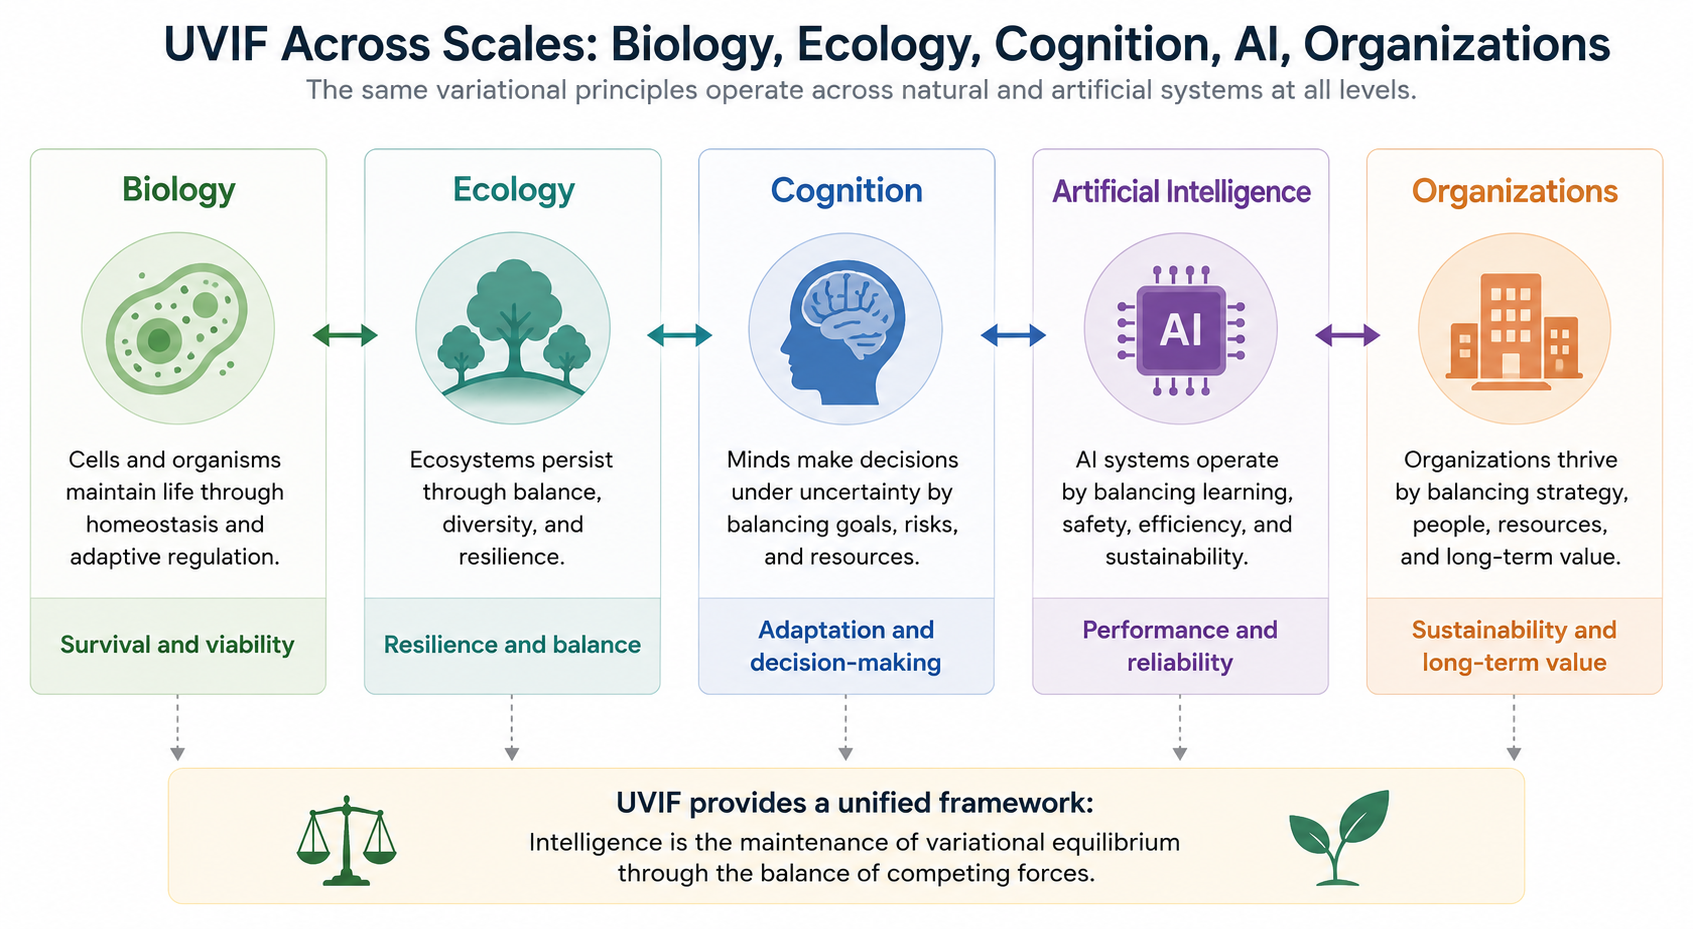
\includegraphics[width=\linewidth]{Figures/Fig5_UVIF_Across_Systems.png}
\caption{UVIF across biological, ecological, cognitive, artificial, and
organizational systems. Although these domains differ in scale and
mechanism, they all maintain functionality through adaptive balance
rather than isolated maximization. UVIF interprets these systems through
a unified variational perspective in which intelligence corresponds to
the maintenance of viable equilibrium under competing pressures,
resource constraints, uncertainty, and environmental change.}
\label{fig:uvif_across_systems}
\end{figure}

The lower part of the figure summarizes the unifying interpretation
provided by \uvif{}. Rather than treating intelligence as isolated
optimization, the framework interprets intelligent operation as the
maintenance of Variational Equilibrium across competing forces. The same
general principle therefore appears across multiple natural and
artificial domains despite their very different physical
implementations.

\subsection{Biological Systems and Physiological Regulation}

The most immediate and compelling validation of the \uvif{} framework
comes from physiology, where the language of force balance and dynamic
equilibrium has described biological function for over a century.

Consider the regulation of blood glucose concentration. The pancreatic
system operates through the opposition of insulin (which drives glucose
into cells, reducing blood concentration) and glucagon (which mobilizes
stored glucose, raising concentration). Neither hormone is simply
maximizing a reward signal; they are opposing forces that jointly
maintain the system within a viable range. When this balance is
disrupted---as in diabetes mellitus---the system fails catastrophically.

In the \uvif{} language, the pancreatic regulatory system instantiates
a Variational Equilibrium: insulin and glucagon correspond to opposing
forces in the force field, and normoglycemia is the equilibrium at
which these forces balance. The admissibility constraints are the
physiological limits beyond which neural and vascular damage occurs.
Adaptive homeostasis corresponds to the shift of the equilibrium
manifold in response to chronic stressors such as chronic
hyperglycemia in diabetes \citep{davies2016adaptive}.

This example generalizes across virtually all physiological regulatory
systems. Thermoregulation balances heat production and dissipation.
Blood pressure regulation balances cardiac output and vascular
resistance. Immune function balances inflammatory and anti-inflammatory
signals. In each case, the system's health is its proximity to
Variational Equilibrium, and disease is the disruption of this
equilibrium \citep{billman2020homeostasis,bich2025homeostasis}.

The evolutionary interpretation is also immediate: organisms that
maintained their Variational Equilibrium across a wide range of
perturbations survived and reproduced; those that were easily
displaced from equilibrium did not. Evolution, in this view, is the
process by which the force field of biological systems has been
refined over billions of years to make Variational Equilibrium
robust \citep{farnsworth2025setpoint,eskov2017homeostasis}.

\subsection{Ecological Systems and Environmental Balance}

Ecosystem dynamics provide the second great testing ground for
\uvif{}. Ecological systems are quintessentially multi-force systems:
predator-prey dynamics, nutrient cycling, competitive exclusion,
mutualism, and succession all involve the opposition and cooperation
of multiple forces acting simultaneously on multiple components
\citep{levin1998ecosystems}.

The canonical predator-prey cycle---where predator and prey
populations oscillate around an equilibrium---is perhaps the simplest
ecological instance of Variational Equilibrium. The predator force
(driving prey population down) and the prey force (driving predator
population down through food limitation) balance at the equilibrium
population densities. The system cycles around this equilibrium rather
than converging to it precisely because biological populations have
finite growth rates and response times---a manifestation of the
homeodynamic principle that equilibria in living systems are dynamic,
not static \citep{lloyd2001homeodynamics}.

More complex ecological systems exhibit higher-dimensional Variational
Equilibria. The spatial self-organization of dryland vegetation
represents a Variational Equilibrium between water competition (a
force driving spatial separation of plants) and facilitation (a force
drawing plants together to share moisture from bare soil)
\citep{kefi2024selforg}. The resulting spatial patterns---bands,
spots, gaps---are the visible signature of this equilibrium, and their
persistence despite ongoing perturbation is evidence of the
equilibrium's stability.

Ecological resilience, in the \uvif{} interpretation, is the size and
robustness of the basin of attraction around the Variational
Equilibrium manifold \citep{gao2016universal,folke2006resilience}.
Systems with high resilience have large basins: they can absorb
significant perturbations and still return to functional equilibrium.
Systems with low resilience are near the edge of their basin: small
perturbations can tip them into a different, possibly dysfunctional,
equilibrium.

The planetary-scale homeostasis hypothesis (the Gaia hypothesis)
represents the most ambitious ecological application of the \uvif{}
framework. The emergence of planetary-scale homeostasis from the
feedback loop between life and the abiotic environment---temperature,
atmospheric composition, ocean chemistry---has been demonstrated in
computational models and provides a striking instance of
self-organized Variational Equilibrium at the highest possible scale
\citep{dyke2013environmental}.

\subsection{Human Cognition and Decision-Making}

Human cognition is the instance of the framework that bears most directly on
the questions of this journal, and it is treated separately and at length in
Section~\ref{sec:cognitive_systems}. In outline, the brain continuously
balances exploration against exploitation, stability against plasticity,
accuracy against metabolic cost, and individual goals against social
constraints; these trade-offs are the cognitive expression of the five
\uvif{} forces, and the manifold along which they are jointly satisfied is the
Variational Equilibrium of cognition.

\subsection{Artificial Intelligence and Adaptive Autonomous Systems}

In artificial intelligence, \uvif{} provides a framework for designing
systems that remain safe, effective, and sustainable across extended
deployment lifetimes. The key insight is that the five forces must all
be explicitly represented in the system's architecture, not collapsed
into a single objective.

A \uvif-aligned AI system for, say, autonomous navigation would not
simply maximize a reward signal for reaching a destination. It would
maintain a force balance between: the epistemic pull to explore
unknown terrain and build better maps; the selective protection of
safety-critical representations (obstacle models, map consistency);
the computational drag that limits onboard processing to available
energy; the action efficiency that selects routes that are both fast
and informative; and the sustainability field that prevents the system
from operating in ways that damage its hardware or deplete its energy
reserves.

The resulting system would not be optimal in the narrow sense of
maximizing any single metric. But it would be robust: capable of
functioning across a wide range of conditions, gracefully degrading
when resources are scarce, and remaining safe even when its models
are uncertain. This is the kind of robustness that the current
paradigm of reward maximization cannot naturally deliver
\citep{garcia2015saferl,yuan2019novel}.

Nature-inspired computing has already drawn on many of these
principles in the design of adaptive algorithms
\citep{jiao2024natureinspired,diaz2025biomimetics}. \uvif{} provides
the unifying theoretical framework that makes these principles coherent
and mutually reinforcing.

\subsection{Societal and Organizational Systems}

The scope of \uvif{} extends naturally to the most complex adaptive
systems that humanity manages: social organizations, institutions,
and economies. These systems face the same fundamental challenge as
biological and ecological systems: how to maintain coherent,
functional operation across time despite continuous internal flux and
external perturbation.

Organizational resilience---the capacity of an institution to absorb
disruption and reorganize while preserving its essential functions---
is the organizational analog of ecological resilience
\citep{ungar2018resilience,folke2006resilience}. Organizations that
achieve long-term resilience do so not by optimizing a single metric
(profit, growth, market share) but by maintaining a force balance
between competing imperatives: efficiency and slack, standardization
and adaptability, short-term performance and long-term investment.

The Integrative Sustainable Intelligence model developed in the
organizational management literature makes a similar argument:
sustainability-oriented organizations must integrate multiple driving
forces rather than subordinating all to a single objective
\citep{silvestre2020integrative,kulkov2023ai}.
Decision-making in organizations that deploy AI must navigate the
competing forces of capability, safety, transparency, and human
oversight \citep{shrestha2019decision}---a challenge that \uvif{}
frames as a problem of maintaining Variational Equilibrium in a
complex socio-technical system.



% Deep revision placeholder inserted.
% [Further conceptual integration recommended]

\section{Relation to Cognitive Theories and Testable Hypotheses}
\label{sec:cognitive_systems}

\subsection{Cognitive interpretation}
\label{subsec:cognition_forces}
For a cognitive implementation, the state might include a belief representation, a policy, retained knowledge, and resource estimates. Epistemic pull then concerns informative sampling; selective protection concerns retention and integrity; computational drag concerns the cost of inference; action efficiency concerns task performance and timeliness; and sustainability concerns future capacity to continue those activities. These are modelling assignments whose separability must be tested.

A cognitive Variational Equilibrium uses the same stationary definition as Eq.~\eqref{eq:veq}. It is not defined as a point where one objective cannot improve without harming another: that would introduce a different, Pareto-based notion. Continuing cognition is more naturally described through trajectories in an admissible operating set, with equilibria relevant only to particular state summaries or fixed conditions.

\subsection{Predictive processing and active inference}
\label{subsec:pp_ai}
Predictive processing emphasizes hierarchical predictions and the updating of beliefs through prediction errors \citep{clark2013whatever}. Active inference provides a generative-model account of perception and action, including epistemic and pragmatic contributions to policy evaluation \citep{friston2010fep,parr2018generalised,parr2022active}. Combining these contributions in one functional does not make them indistinguishable or imply that their behavioural balance must be fixed. That balance depends on beliefs, preferences, policies, and the model's treatment of the environment and internal states.

\uvif{} makes a different organizational choice by assigning named update components to regulatory demands. This may facilitate intervention and reporting, but it is not yet a derivation of a distinct class of behaviour. In particular, a resource-induced change in exploration is not by itself evidence against active inference: an active-inference model that represents resource state may also predict it. A valid comparison must identify which variables and mechanisms each fitted model includes.

Likewise, a common active-inference formulation may omit a detailed account of inference expenditure without that omission being an impossibility of the framework. The pertinent comparison is between specified models with and without explicit computational and reserve accounting. Claims about entire theoretical families would exceed what the present framework establishes.

\subsection{Resource-rational analysis}
\label{subsec:resource_rational}
Resource-rational analysis explains cognitive strategies in terms of expected benefits relative to computational costs \citep{lieder2019resourcerational,griffiths2015rational}. Human planning studies provide examples of how such models can be tested \citep{callaway2022rational}. This literature directly anticipates the interaction between action efficiency and computational drag.

The proposed sustainability component asks whether the resource state carried between decisions changes the preferred computation policy. A per-task model that omits those dynamics may fail, but an extended resource-rational model can represent them. Irreversible outcomes can similarly be represented through absorbing states, constraints, or preferences. UVIF's possible contribution is a convenient decomposition and independently measurable mechanisms, not the exclusive ability to represent these considerations.

\subsection{Allostasis and cognitive architectures}
\label{subsec:allostasis}
Allostasis concerns predictive physiological regulation \citep{schulkin2019allostasis}. Evidence for a large-scale brain system supporting allostasis and interoception motivates examining cognition and bodily regulation together \citep{kleckner2017evidence}. It does not establish a one-to-one mapping between a neural network and the five proposed forces. Such a mapping would require independent measurements and interventions.

\label{subsec:architectures}
Integrated cognitive architectures describe mechanisms for memory, learning, control, and action \citep{laird2017standard,kotseruba201840}. \uvif{} is a proposed regulatory description that could be implemented within such architectures. It does not specify a complete cognitive architecture. A concrete implementation must explain how component signals are computed, how competing updates are resolved, and how the computation used by the regulatory layer itself is charged to the resource budget.

\subsection{Comparative hypotheses}
\label{subsec:cog_predictions}
The following hypotheses concern specified implementations rather than unique predictions of UVIF as a whole. Their value lies in enabling controlled comparisons and revealing when the additional decomposition is unnecessary.

\begin{enumerate}[label=(H\arabic*),leftmargin=2.4em]
\item \textbf{Resource-dependent allocation.} Manipulating available computation, time, or reserve state while preserving external task information and rewards should alter information acquisition when the specified model couples allocation to those resources. Compare a resource-responsive UVIF model with both fixed-weight and resource-responsive alternatives. Measure sampling decisions, response time, task performance, and resource expenditure. A failure to improve held-out prediction over equally flexible alternatives would weaken the case for the proposed decomposition.

\item \textbf{Effects of resource carry-over.} When expenditure reduces capacity in later episodes, a model that tracks reserves should predict different allocation from an otherwise comparable model that resets resources after each episode. Match the observed task and state information across agents, and compare with a long-horizon resource-rational or constrained-control model. The prediction concerns explicit carry-over dynamics, not an assumed distinction between a sustainability force and all possible long-horizon utilities.

\item \textbf{Protection under irreversible outcomes.} Compare a hard admissibility mechanism with calibrated soft penalties under the same transition model, including irreversible states. Measure violation frequency, retained task performance, and unnecessary refusal. Hard and soft formulations may coincide over a bounded range of payoffs; the experiment must report that range. No behavioural observation here establishes impossibility of representation by every utility model.

\item \textbf{Component ablation.} Remove one implemented component while preserving observations and evaluating both fixed-parameter and retuned controls. Predefine the expected consequence: reduced learning under epistemic ablation, greater damage under protection ablation, or reserve depletion under sustainability ablation. Effects need not be monotonic or unique, because other components may compensate. An ablation is informative only when it tests an independently meaningful mechanism rather than a failure built into the outcome definition.
\end{enumerate}

Section~\ref{sec:future} specifies common evaluation requirements. This paper does not report tests of H1--H4 or claim that they distinguish UVIF from every member of the comparator families. The companion repository provides an executed notebook and saved outputs for illustrative policy-grid demonstrations \citep{Hamam2026GitHub}. Its implementation maximizes a scalar score formed from the five named contributions, rather than integrating Eq.~\eqref{eq:projected}, and the notebook records two negative results that bear directly on the hypotheses above. First, a fixed unit-weight scalarization over the same state-dependent component functions reproduces every policy that implementation selects, across all declared environments; the implementation is therefore a scalar optimization and cannot evidence a departure from one. Second, a finite monotone hinge penalty on exposure above the admissibility threshold reproduces the constrained policies exactly over the same declared set, which refutes any claim that constrained choice under irreversibility is irreducible to a finite monotone penalty. Both results are exhaustive over the declared environment set and policy grid. They are reported as demonstrations of what that implementation cannot establish, and they motivate the evaluation requirements of Section~\ref{sec:future}; neither the notebook nor this paper validates H1--H4 or the vector-field model.

\section{Hypothetical Design Scenarios}
\label{sec:case_studies}

The following scenarios illustrate how the vocabulary could guide design and evaluation. They are not case studies with collected data, implemented controllers, or demonstrated benefits. Each requires a domain-specific model and comparison with established practice.

\subsection{Clinical decision support}
A decision-support system may have to allocate further assessment while accounting for uncertainty, clinician workload, and the consequences of delay. Epistemic pull could represent the expected decision value of an additional observation; selective protection could concern integrity of the patient record and validated model components; computational drag could track inference latency and processing cost; action efficiency could represent timely decision support; and sustainability could track review capacity across a sequence of cases.

Clinical test costs and burdens should not be conflated with computation costs: they belong in the explicitly defined action and resource model. Clinical eligibility, escalation rules, and patient safety requirements would be externally specified constraints. No treatment recommendation or clinical benefit follows from the force metaphor. Evaluation would require clinical oversight, relevant approvals, and evidence that the model improves appropriate outcomes over validated decision-support baselines.

\subsection{Energy management}
For a resource-limited infrastructure controller, a candidate state includes reserve capacity, predicted demand, equipment condition, and available computation. The proposed decomposition separates forecasting, preservation of critical components, computation expenditure, dispatch performance, and future supply capacity. Existing optimization methods can represent these quantities; UVIF would need to show that its decomposition improves monitoring, adaptation, or diagnosis.

A useful comparison would apply identical demand sequences, reserve models, actuator limits, and forecast information to the competing controllers. Outcomes would include unmet demand, constraint violations, computational burden, and reserve depletion over a declared horizon. A favourable average cost would not compensate for an unreported violation of a hard operational requirement.

\subsection{Autonomous transportation}
The navigation example in Section~\ref{sec:optimization_equilibrium} can be extended to sensor allocation and memory updates. A UVIF implementation would need an explicit transition model, a way to connect policy updates to vehicle controls, and a safety mechanism that respects physical braking and sensing limitations. Equilibrium-seeking dynamics alone do not ensure recovery from an obstacle or sensor failure.

Testing should separate normal operation, known disturbances, and conditions outside the assumed model. Task completion, reserve use, intervention frequency, and failures should be reported together. Comparators should include resource-aware constrained planning or control, not only a controller optimized for travel speed.

\subsection{Cybersecurity}
A monitoring system may allocate inspection effort between immediate threat detection and sustained availability. The components could represent information gathering, protection of keys and logs, inspection expenditure, response effectiveness, and future monitoring capacity. A threat model must state attacker capabilities and which assets are protected. No architectural label makes a system resistant to adversarial inputs.

Ablations could examine whether an explicit capacity model reduces overload under repeated alerts, while retaining detection performance. Both missed threats and disruptions to legitimate activity matter. Tuning the protective component only on attacks used for evaluation would invalidate the intended comparison.

\subsection{Organizational capacity}
A service organization may balance information gathering, retention of expertise, processing effort, timely service, and future staffing capacity. Here the central modelling issue is governance: whose workload, risk, and service quality count, and who may alter the constraints? A persistent organization can still impose unacceptable costs on its members or clients.

The framework can make these trade-offs explicit, but it cannot select legitimate priorities on its own. Evaluation would require stakeholder-defined outcomes and comparisons with existing capacity-planning methods. Institutional longevity is not an adequate sole measure of success.

\section{Comparative Methodological Positioning}
\label{sec:comparative}

Table~\ref{tab:comparison} separates mathematical methods, learning frameworks, and organizational descriptions. They operate at different levels and should not be ranked as if each were a complete alternative to the others.

\begin{table}[tbp]
\centering
\renewcommand{\baselinestretch}{1}\small
\renewcommand{\arraystretch}{1.25}
\caption{Scope of comparison. The final column identifies what a UVIF evaluation must establish, rather than assigning unsupported superiority scores.}
\label{tab:comparison}
\begin{tabularx}{\linewidth}{@{}>{\raggedright\arraybackslash}p{2.9cm}YY@{}}
\toprule
Approach & Relevant capability & Requirement for a UVIF comparison \\
\midrule
Constrained and multi-objective optimization & Explicit trade-offs, constraints, multiple criteria & Show value beyond relabelling objectives or adapting weights \\
Safe reinforcement learning & Sequential learning with risk and safety considerations & Match observations, constraints, horizons, and training resources \\
Active inference & Generative-model treatment of action and information acquisition & Compare fully specified resource-aware models \\
Resource-rational analysis & Benefits of cognition relative to computation costs & Include reserve carry-over and equivalent planning opportunities \\
Allostatic regulation & Anticipatory regulation of internal conditions & Test an independently measurable five-component mapping \\
Cognitive architectures & Integrated mechanisms for memory, learning, and action & Specify and measure the cost of the added regulatory layer \\
\uvif{} & Proposed explicit five-component decomposition & Establish identifiability, tractability, and incremental predictive value \\
\bottomrule
\end{tabularx}
\end{table}

\subsection{Optimization and learning as possible implementations}
Equation~\eqref{eq:toy_potential} demonstrates that one valid UVIF instance is also an optimization system. A multi-objective interpretation, a constrained policy search, or a learning-based controller may therefore implement the proposed organization. UVIF should not be distinguished solely by the use of several considerations or by adaptive weighting, both of which can be represented within established mathematical frameworks.

Reinforcement learning provides methods for learning from sequential interaction, while safe RL addresses additional risk and constraint requirements \citep{garcia2015saferl}. The question for UVIF is whether its explicit assignment of regulatory roles improves specification, transfer, or failure diagnosis under a fair comparison. A hard constraint can be a stronger protection mechanism than a soft force; describing it as external does not make it less effective.

Data-driven models likewise use explicit training objectives, even when the learned representations are not readily interpretable. Such models could supply prediction, perception, or value estimates inside a UVIF implementation. The regulatory decomposition does not by itself render their representations interpretable or improve generalization.

\subsection{The intended level of novelty}
The proposed contribution is a modelling discipline: name the regulatory demands, assign measurable state-dependent mechanisms to them, distinguish costs from constraints, and evaluate persistence together with task performance. It remains possible that a smaller decomposition, an established architecture, or a single well-specified objective will provide an equally good or better account.

Demonstrating novelty requires more than broad applicability. It requires a case in which the decomposition supports a useful measurement, intervention, prediction, or design decision that is difficult to obtain from a comparably explicit baseline. The current paper motivates that programme and gives a consistent template; it does not establish that the requirement has been met empirically.

\section{Implications for Evaluation and Interpretation}
\label{sec:implications}

\subsection{Persistence must be measured alongside performance}
A regulatory framework should be evaluated across time, not only at a final task score. Useful outcomes include task quality, decision latency, resource expenditure, retention of prior competence, constraint violations, and recovery following a specified disturbance. Reporting these quantities separately prevents an aggregate score from hiding an operationally important failure.

For a known stationary model, distance to a stable equilibrium may help characterize recovery. In a dynamic task, that distance can be misleading: a useful action may move the system away from a frozen equilibrium, and a failing system may have a small net update because it is stuck. Equilibrium proximity is therefore a model-dependent diagnostic rather than a general intelligence metric.

\subsection{Accounting for the regulatory layer}
Computing information gain, estimating risk, monitoring reserves, and adapting weights all incur costs. These must be included in the same budget used to evaluate the agent. Otherwise an apparently resource-aware design can receive an unreported computational advantage. Model calibration and online operation should also be distinguished: expensive offline fitting does not have the same implications as an expensive real-time decision rule.

The five components should support diagnosis only where the mapping from observables to mechanisms is justified. A decline in performance cannot be attributed to the sustainability component merely because it occurs late in a deployment. Alternative explanations include distribution shift, memory corruption, and changing task difficulty. Controlled perturbations and held-out predictions are needed to separate them.

\subsection{Persistence is not a complete account of intelligence}
Stability and viability are relevant to sustained cognitive performance, but they do not explain all learning, reasoning, representation, or social understanding. Some intelligent actions deliberately leave a familiar operating regime. A system can also remain stable while pursuing harmful or irrelevant objectives. UVIF should therefore complement task- and context-specific accounts of cognition, rather than replace them with an unrestricted definition based on equilibrium.

\section{Limitations and Open Challenges}
\label{sec:limitations}

\subsection{The decomposition is posited and may not be identifiable}
The five components are motivated by recurring design concerns, not derived as necessary or sufficient constituents of intelligence. Other decompositions may be equally useful. If a vector field is added to one component and subtracted from another, the net dynamics can remain unchanged. Observing trajectories alone consequently need not identify the components. Independent measurements, structural restrictions, or interventions are required before a force label can be given a causal interpretation.

Overlapping cost measures create a related problem. Energy may appear in both computational drag and sustainability, and protection may overlap with risk constraints. A model must explain whether these terms represent distinct timescales, distinct consequences, or deliberate multiple valuation. Without that explanation, apparent advantages may reflect repeated penalties rather than a new mechanism.

\subsection{The mathematical formulation is restricted}
The projected dynamics assumes a continuous state, directly selectable first-order updates, and a fixed convex feasible set. Real systems may have discrete modes, nonconvex constraints, delayed observations, and limited control authority. Existence of an equilibrium, stability, robustness, and tracking do not follow from the force labels. The analytical example establishes those properties only for its scalar linear field and fixed parameters.

A general variational functional has not been derived. It would be misleading to infer a common principle of stationary action from the proposed notation. Extensions to stochastic systems would also need probabilistic definitions of constraint satisfaction and persistence, with explicit disturbance assumptions and time horizons.

\subsection{Empirical and comparative support is absent}
This manuscript reports no new experiment or validated simulation comparison. The companion repository contains illustrative simulations with stipulated objectives and restricted comparators (Section~\ref{subsec:cog_predictions}). H1--H4 describe a prospective evaluation programme; they are not demonstrated effects. Neither the clinical and engineering scenarios nor the biological analogies provide independent validation. The lack of evidence for incremental value over resource-aware alternatives is the principal obstacle to presenting UVIF as an established theory or proven architecture.

The literature discussion is selective. A more comprehensive account should examine viability theory, adaptive and robust control, constrained decision processes, and related dynamical approaches to cognition in depth. Any claim of priority or formal generalization would require that comparison and a precise derivation.

\subsection{Normative and cross-domain limitations}
Admissibility specifications may omit important harms or encode contested priorities. Mathematical feasibility is not a substitute for domain expertise, governance, or ethical judgment. Persistent operation is not inherently desirable, and natural systems provide no automatic standard for acceptable artificial behaviour.

Broad domain translation also risks becoming unfalsifiable if every outcome can be redescribed as a change in force balance. To limit that risk, an application must specify the component measurements, parameter rules, and predicted outcomes before evaluation. A result inconsistent with those commitments should count against that implementation, rather than being absorbed by unconstrained redefinition of its fields.

% ============================================================
%  Section 10 – Future Research Directions
% ============================================================
\section{Future Research Directions}
\label{sec:future}

The limitations identified in Section~\ref{sec:limitations} define the
boundaries of the current \uvif{} contribution and, simultaneously, the
agenda for its further development. We outline five research directions
that we consider most pressing.

\begin{figure}[!t]
\centering
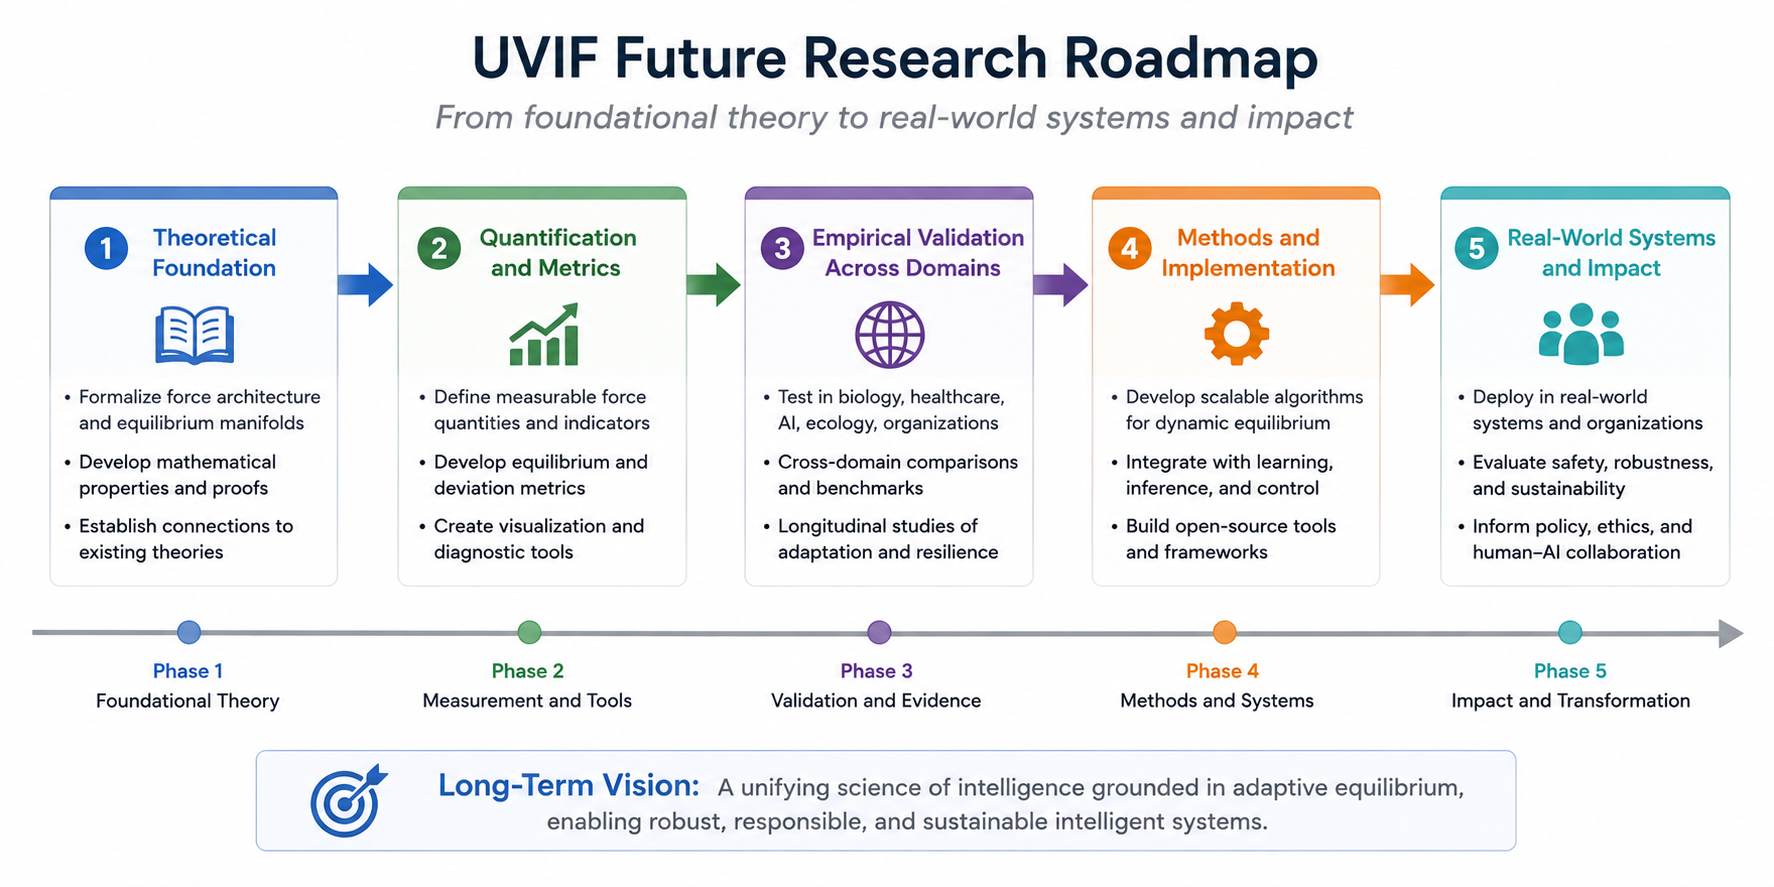
\includegraphics[width=\linewidth]{Figures/Fig10_Future_Roadmap.png}
\caption{UVIF future research roadmap. The framework evolves through
five major stages: theoretical formalization, equilibrium quantification,
cross-domain empirical validation, scalable implementation, and
real-world deployment. The long-term objective is the development of a
unified science of intelligence grounded in adaptive equilibrium,
bounded knowledge, sustainability, and persistent viability.}
\label{fig:future_roadmap}
\end{figure}

Fig.~\ref{fig:future_roadmap} presents a structured roadmap for the
future development of \uvif{}. The figure emphasizes that the framework
should not remain only a conceptual philosophy of intelligence. Rather,
it should progressively evolve into a mathematically grounded,
empirically validated, and operationally deployable scientific
framework.

The first stage concerns \emph{theoretical foundation}. Future work
must formalize the geometry of Variational Equilibrium manifolds,
rigorously define force interactions, establish stability properties,
and connect \uvif{} with existing mathematical theories of dynamical
systems, variational flows, stochastic processes, and viability
analysis.

The second stage focuses on \emph{quantification and metrics}. The
framework will require measurable quantities capable of estimating force
balance, equilibrium proximity, system deviation, adaptive resilience,
and sustainability under changing conditions. These metrics will be
necessary for transforming \uvif{} from a qualitative framework into a
testable scientific methodology.

The third stage involves \emph{empirical validation across domains}.
One of the defining characteristics of \uvif{} is its cross-domain
scope. Consequently, future research must evaluate the framework across
biology, healthcare, artificial intelligence, ecology, cognition, and
organizational systems in order to determine whether the proposed
organizational principles consistently emerge in real-world adaptive
systems.

The fourth stage concerns \emph{methods and implementation}. This stage
includes the development of scalable algorithms, equilibrium-aware AI
architectures, adaptive control mechanisms, uncertainty-aware decision
systems, and computationally sustainable intelligent systems capable of
maintaining dynamic equilibrium under partial observability and noisy
environments.

The fifth stage represents \emph{real-world systems and impact}. The
long-term vision of \uvif{} is not merely theoretical elegance, but the
development of safer, more sustainable, more resilient, and more
human-compatible intelligent systems capable of operating coherently
under uncertainty, changing environments, and long temporal horizons.

The roadmap shown in the figure also reinforces an important conceptual
point of this paper: the development of intelligence research may
require a transition away from isolated short-term optimization and
toward adaptive equilibrium, bounded knowability, sustainability, and
persistent viability as central organizational principles.

\subsection{PDE-Based Variational Dynamics}

The most natural mathematical language for \uvif{} in spatially
extended systems is that of partial differential equations (PDEs).
Many of the systems to which \uvif{} applies---ecosystems, neural
fields, social networks---have structure in space as well as time,
and the Variational Equilibrium of such systems is a spatial pattern,
not just a single configuration.

The mathematical theory of variational methods for evolution---
encompassing gradient flows, free energy functionals, and metric-space
geometry \citep{campos2021discrete}---provides the starting point
for this development. The challenge is to formulate the five forces
of \uvif{} as terms in a PDE system in a way that is both
mathematically tractable and phenomenologically faithful to the
systems being modeled.

A promising approach is to formulate the force dynamics as a
gradient flow on a suitable state space, where the energy functional
captures the five forces and the Variational Equilibrium is the
minimizer of this functional. Existence and regularity of solutions
can then be studied using tools from the theory of evolution equations
in Banach and Hilbert spaces. The connection to the variational methods
for ecosystem dynamics studied in ecology \citep{kefi2024selforg,
rietkerk2021evasion} and the free-energy dynamics studied in
neuroscience \citep{friston2010fep,kim2022freeenergy} will be
particularly fruitful.

\subsection{Nature-Inspired Adaptive AI Architectures}

The second research direction is the engineering of AI architectures
that explicitly instantiate the \uvif{} force balance. Current
architectures---transformers, convolutional networks, recurrent
networks---are designed around the efficient implementation of
specific computational operations, not around the maintenance of
a force balance. Building \uvif{}-aligned architectures requires
rethinking the structure of learning systems from the ground up.

Promising directions include:
\begin{itemize}[leftmargin=1.5em]
  \item \emph{Modular architectures} that separate the components
    responsible for epistemic pull (active learning, uncertainty
    estimation), selective protection (knowledge consolidation, memory
    replay), computational efficiency (pruning, sparse computation),
    and sustainability (resource monitoring, adaptive computation).
  \item \emph{Intrinsic motivation mechanisms} that implement the
    epistemic pull force as an endogenous reward for information gain,
    integrated with extrinsic task performance signals
    \citep{friston2017curiosity,dubey2019curiosity}.
  \item \emph{Biomimetic regularization} schemes that implement
    selective protection by drawing on the biological principles of
    synaptic consolidation, replay, and homeostatic plasticity
    \citep{moreddu2025bioinspired,diaz2025biomimetics}.
\end{itemize}

The green AI literature provides an important constraint: the
architectures developed should be evaluated not only for their
performance but for their energy efficiency and computational
sustainability \citep{bolon2024greenai}. A \uvif{}-aligned architecture
that requires massive computational resources to maintain its force
balance has failed to instantiate the computational drag force
adequately.

\subsection{Multi-Agent Equilibrium Systems}

The third research direction extends \uvif{} from single-agent to
multi-agent systems. When multiple \uvif{}-aligned agents interact,
the system-level Variational Equilibrium is not simply the sum of
the individual agents' equilibria; it is a collective configuration
that emerges from the interactions between agents, each pursuing its
own force balance.

The natural theoretical framework for this extension is
game theory. Multi-agent Nash equilibria \citep{semsar2009multiagent,
wang2022cooperative} provide the micro-level mechanism by which
macro-level Variational Equilibria are generated in multi-agent
systems. The challenge is to design individual agent force architectures
such that the resulting Nash equilibria are close to the socially
optimal Variational Equilibrium---the configuration that maximizes
the collective force balance \citep{memarzadeh2020food}.

This is a multi-agent analog of the alignment problem in AI safety:
how can individually rational agents be designed so that their
collective behavior is beneficial? The \uvif{} framework suggests that
the answer lies in giving each agent a sustainability force that is
sensitive to the collective system's resource use, so that individual
agents are naturally incentivized to avoid behaviors that deplete the
shared environment.

Ecological models of co-evolutionary dynamics---where organisms evolve
strategies that are individually adaptive and collectively sustainable
---provide empirical inspiration for this research direction
\citep{levin1998ecosystems,dyke2013environmental}. The theoretical
tools of evolutionary game theory, mean-field games, and cooperative
game theory will all be relevant.

\subsection{Sustainable and Self-Regulating Intelligence}

The fourth research direction is the development of AI systems that
actively maintain their own Variational Equilibrium---systems that
are not only designed with the force balance in mind but that monitor
their own operating configuration and take corrective action when
displaced from equilibrium.

This is the AI analog of biological self-regulation: the capacity
of a living system to detect deviations from homeostatic set-points
and deploy corrective responses. In artificial systems, it requires:
\begin{itemize}[leftmargin=1.5em]
  \item \emph{Force monitoring}: mechanisms that estimate the current
    values of the five forces from observable system behavior.
  \item \emph{Equilibrium detection}: methods for determining whether
    the current state is within the basin of attraction of the
    Variational Equilibrium.
  \item \emph{Corrective dynamics}: algorithms that, upon detecting
    displacement from equilibrium, modulate the system's behavior
    to restore the force balance.
\end{itemize}

The free-energy principle's account of allostasis---the active
adjustment of set-points in response to anticipated perturbations
---provides a starting point for the third component
\citep{bettinger2023physiological,kim2022freeenergy}. Adaptive
homeostasis in biology, where the homeostatic range expands or
contracts in response to sub-threshold stimuli, provides a model
for how set-point adaptation can be incorporated into the \uvif{}
dynamics \citep{davies2016adaptive}.

\subsection{Toward Unified Organizational Theories of Intelligence}

The fifth research direction is the most ambitious: the development
of a genuinely unified theory of intelligence that subsumes the
biological, ecological, cognitive, artificial, and organizational
domains within a single formal framework.

Such a theory would need to:
\begin{itemize}[leftmargin=1.5em]
  \item Provide formal definitions of the five \uvif{} forces that
    are applicable across all domains, together with domain-specific
    instantiations.
  \item Derive quantitative predictions about the relationship between
    force balance and system performance (intelligence, health,
    resilience, sustainability) in each domain.
  \item Show that existing domain-specific theories
    (homeostasis, ecological resilience, free-energy principle,
    organizational learning) are special cases of or can be embedded
    within the \uvif{} framework.
  \item Identify universal signatures of Variational Equilibrium
    that can be observed across domains---metrics that indicate
    proximity to equilibrium regardless of the specific system
    being studied.
\end{itemize}

The unification of theories that have developed in relative isolation
is one of the most challenging and most productive activities in
science. The history of science offers many examples---statistical
mechanics unifying thermodynamics and atomic theory; the modern
synthesis unifying genetics and evolution; quantum electrodynamics
unifying quantum mechanics and electromagnetism---of unifications
that transformed entire fields. The \uvif{} framework is proposed
in this spirit: as a candidate for the unifying framework that the
science of intelligence---biological, artificial, and organizational---
currently lacks.



% Deep revision placeholder inserted.
% [Further conceptual integration recommended]

\section{Conclusion}
\label{sec:conclusion}

UVIF proposes an explicit decomposition of five regulatory demands relevant to persistent cognitive systems: information acquisition, selective protection, computation cost, effective action, and future operating capacity. The present formulation distinguishes these soft influences from hard admissibility requirements and separates stationary equilibrium from invariant operation and adaptation under changing conditions.

The analytical example demonstrates stability in one restricted model and also shows that its dynamics can minimize a scalar objective. The contribution is therefore a proposed organization of modelling responsibilities, not a demonstrated replacement for optimization. Its relationship to active inference, resource-rational analysis, allostasis, and cognitive architectures is potentially complementary.

The decisive next step is a controlled comparison in which the components are independently specified, their computational costs are counted, and their predictions are tested against capable alternatives. Until such evidence is available, UVIF should be treated as a conceptual research programme whose usefulness, component structure, and range of applicability remain open to revision.

\section*{Data availability}
No empirical datasets are reported in this conceptual study. The analytical example is specified in full in Section~\ref{subsec:example}. Companion policy-grid simulation code and saved outputs are publicly accessible in the versioned repository \citep{Hamam2026GitHub}. Those illustrative simulations are distinct from the revised vector-field formulation and do not establish the comparative hypotheses as validated findings.
\section*{CRediT author contribution statement}
\textbf{Habib Hamam:} Conceptualization, Methodology, Formal analysis, Investigation, Writing -- original draft, Writing -- review \& editing.
\section*{Funding}
This work was supported by Universit\'e de Moncton, University of Johannesburg, IITG, and CRSNG/NSERC under Grant RGPIN-2025-05918.
\section*{Acknowledgments}
The author acknowledges the support of the affiliating institutions for facilitating this research.
\section*{Declaration of competing interest}
The author declares that they have no known competing financial interests or personal relationships that could have influenced the work reported in this paper.
\section*{Ethics statement}
Not applicable. This conceptual study reports no research involving human participants or animals.
\section*{Declaration of generative AI and AI-assisted technologies in the manuscript preparation process}
OpenAI Codex (GPT-6) was used to assist with critical review, restructuring, language revision, mathematical consistency checks, LaTeX editing, and preparation of the schematic diagrams. The author is responsible for independently verifying the arguments, equations, references, and figures and for approving the final manuscript.
% Before submission, confirm completed author review and disclose any other AI tools used.
\bibliographystyle{elsarticle-num}
\bibliography{Sections/References}
\end{document}
